\documentclass[conference]{IEEEtran}
%DIF LATEXDIFF DIFFERENCE FILE
%DIF DEL /tmp/PU2VPE45Xt/latexdiff-vc-34a97a8d8868555507dd875f30368a64cb8b20eb/BadUSBC.tex   Fri Mar 12 15:55:21 2021
%DIF ADD BadUSBC.tex                                                                         Mon Mar 22 19:40:14 2021
\IEEEoverridecommandlockouts
% The preceding line is only needed to identify funding in the first footnote. If that is unneeded, please comment it out.

\makeatletter
\def\lst@makecaption{%
  \def\@captype{table}%
  \@makecaption
}
\makeatother

\newcommand{\tool}{\mbox{\textsc{BadUSB-C}}\xspace}

\newcommand{\outline}[1]{}
\newcommand{\mytodocyan}[1]{}


\newcommand{\hongyi}[1]{}
\newcommand{\mytodopink}[1]{}

\newcommand{\shuqing}[1]{}
\newcommand{\mytodopurple}[1]{}

\newcommand{\yechang}[1]{}
\newcommand{\mytodored}[1]{}

\newcommand{\linyou}[1]{}
\newcommand{\mytodoblue}[1]{}

\newcommand{\chaozu}[1]{}
\newcommand{\mytodogrey}[1]{}
\usepackage{enumerate}
\usepackage[shortlabels]{enumitem}

\newcommand{\fengwei}[1]{}

\newcommand{\mycircled}[1]{%
	\begin{tikzpicture}[baseline={(char.base)}]
		\node (char) {\small{#1}};
		\node[draw,circle,minimum size=10,inner sep=0pt,overlay] (char.center){};
	\end{tikzpicture}
}
\usepackage{textcomp}

\usepackage{tikz,pgf}
\usetikzlibrary{calc}
\makeatletter
\def\mfontsize{\f@size}
\newcommand{\circled[2]}{
	\tikzset{mystyle/.style={circle,#1,minimum size=10,inner sep=0pt}}
	\tikz[baseline=-3pt]
	{
		\node[mystyle] (char.center) {\vphantom{WAH1g}#2};
	}
}
\makeatother

\definecolor{myyellow}{RGB}{237,125,49}
\definecolor{myblue}{RGB}{91,155,213}

\usepackage[breaklinks=true,hidelinks,colorlinks=true,citecolor=blue,urlcolor=black,linkcolor=purple]{hyperref}
\usepackage{balance}

\usepackage{xspace}
\usepackage{cite}
\usepackage{amsmath,amssymb,amsfonts}
\usepackage{graphicx}
\usepackage{textcomp}
\usepackage{xcolor}
\usepackage{hyperref}
\usepackage{threeparttable}
\usepackage{colortbl}
\usepackage{graphicx}
\usepackage{listings}
\usepackage{color}
\usepackage{array}
\usepackage{float}
\usepackage{graphicx}
\usepackage{subfigure}
\usepackage{multirow}
\usepackage{colortbl}
\usepackage[linesnumbered,boxed]{algorithm2e}
\usepackage{algpseudocode}
\usepackage{framed}
\setlength\FrameSep{0.5em}
\usepackage{pifont}
\usepackage{enumitem}
\usepackage{balance}
\usepackage{url}
\usepackage[T1]{fontenc}
\usepackage[utf8]{inputenc}
\usepackage[font=small,labelfont=bf,tableposition=top]{caption}
\usepackage{booktabs}
\usepackage{tabularx}
\usepackage{diagbox}
\usepackage{algpseudocode}
\usepackage{amsmath}
\usepackage{listings}
\usepackage{makecell}
\usepackage{verbatim}
\usepackage{acronym}
\usepackage[super]{nth}

\lstset{
	frame=single,
	breaklines,
	language=python,
	basicstyle=\small,
}


\def\BibTeX{{\rm B\kern-.05em{\sc i\kern-.025em b}\kern-.08em
    T\kern-.1667em\lower.7ex\hbox{E}\kern-.125emX}}
%DIF PREAMBLE EXTENSION ADDED BY LATEXDIFF
%DIF UNDERLINE PREAMBLE %DIF PREAMBLE
\RequirePackage[normalem]{ulem} %DIF PREAMBLE
\RequirePackage{color}\definecolor{RED}{rgb}{1,0,0}\definecolor{BLUE}{rgb}{0,0,1} %DIF PREAMBLE
\providecommand{\DIFaddtex}[1]{{\protect\color{blue}\uwave{#1}}} %DIF PREAMBLE
\providecommand{\DIFdeltex}[1]{{\protect\color{red}\sout{#1}}}                      %DIF PREAMBLE
%DIF SAFE PREAMBLE %DIF PREAMBLE
\providecommand{\DIFaddbegin}{} %DIF PREAMBLE
\providecommand{\DIFaddend}{} %DIF PREAMBLE
\providecommand{\DIFdelbegin}{} %DIF PREAMBLE
\providecommand{\DIFdelend}{} %DIF PREAMBLE
\providecommand{\DIFmodbegin}{} %DIF PREAMBLE
\providecommand{\DIFmodend}{} %DIF PREAMBLE
%DIF FLOATSAFE PREAMBLE %DIF PREAMBLE
\providecommand{\DIFaddFL}[1]{\DIFadd{#1}} %DIF PREAMBLE
\providecommand{\DIFdelFL}[1]{\DIFdel{#1}} %DIF PREAMBLE
\providecommand{\DIFaddbeginFL}{} %DIF PREAMBLE
\providecommand{\DIFaddendFL}{} %DIF PREAMBLE
\providecommand{\DIFdelbeginFL}{} %DIF PREAMBLE
\providecommand{\DIFdelendFL}{} %DIF PREAMBLE
%DIF HYPERREF PREAMBLE %DIF PREAMBLE
\providecommand{\DIFadd}[1]{\texorpdfstring{\DIFaddtex{#1}}{#1}} %DIF PREAMBLE
\providecommand{\DIFdel}[1]{\texorpdfstring{\DIFdeltex{#1}}{}} %DIF PREAMBLE
\newcommand{\DIFscaledelfig}{0.5}
%DIF HIGHLIGHTGRAPHICS PREAMBLE %DIF PREAMBLE
\RequirePackage{settobox} %DIF PREAMBLE
\RequirePackage{letltxmacro} %DIF PREAMBLE
\newsavebox{\DIFdelgraphicsbox} %DIF PREAMBLE
\newlength{\DIFdelgraphicswidth} %DIF PREAMBLE
\newlength{\DIFdelgraphicsheight} %DIF PREAMBLE
% store original definition of \includegraphics %DIF PREAMBLE
\LetLtxMacro{\DIFOincludegraphics}{\includegraphics} %DIF PREAMBLE
\newcommand{\DIFaddincludegraphics}[2][]{{\color{blue}\fbox{\DIFOincludegraphics[#1]{#2}}}} %DIF PREAMBLE
\newcommand{\DIFdelincludegraphics}[2][]{% %DIF PREAMBLE
\sbox{\DIFdelgraphicsbox}{\DIFOincludegraphics[#1]{#2}}% %DIF PREAMBLE
\settoboxwidth{\DIFdelgraphicswidth}{\DIFdelgraphicsbox} %DIF PREAMBLE
\settoboxtotalheight{\DIFdelgraphicsheight}{\DIFdelgraphicsbox} %DIF PREAMBLE
\scalebox{\DIFscaledelfig}{% %DIF PREAMBLE
\parbox[b]{\DIFdelgraphicswidth}{\usebox{\DIFdelgraphicsbox}\\[-\baselineskip] \rule{\DIFdelgraphicswidth}{0em}}\llap{\resizebox{\DIFdelgraphicswidth}{\DIFdelgraphicsheight}{% %DIF PREAMBLE
\setlength{\unitlength}{\DIFdelgraphicswidth}% %DIF PREAMBLE
\begin{picture}(1,1)% %DIF PREAMBLE
\thicklines\linethickness{2pt} %DIF PREAMBLE
{\color[rgb]{1,0,0}\put(0,0){\framebox(1,1){}}}% %DIF PREAMBLE
{\color[rgb]{1,0,0}\put(0,0){\line( 1,1){1}}}% %DIF PREAMBLE
{\color[rgb]{1,0,0}\put(0,1){\line(1,-1){1}}}% %DIF PREAMBLE
\end{picture}% %DIF PREAMBLE
}\hspace*{3pt}}} %DIF PREAMBLE
} %DIF PREAMBLE
\LetLtxMacro{\DIFOaddbegin}{\DIFaddbegin} %DIF PREAMBLE
\LetLtxMacro{\DIFOaddend}{\DIFaddend} %DIF PREAMBLE
\LetLtxMacro{\DIFOdelbegin}{\DIFdelbegin} %DIF PREAMBLE
\LetLtxMacro{\DIFOdelend}{\DIFdelend} %DIF PREAMBLE
\DeclareRobustCommand{\DIFaddbegin}{\DIFOaddbegin \let\includegraphics\DIFaddincludegraphics} %DIF PREAMBLE
\DeclareRobustCommand{\DIFaddend}{\DIFOaddend \let\includegraphics\DIFOincludegraphics} %DIF PREAMBLE
\DeclareRobustCommand{\DIFdelbegin}{\DIFOdelbegin \let\includegraphics\DIFdelincludegraphics} %DIF PREAMBLE
\DeclareRobustCommand{\DIFdelend}{\DIFOaddend \let\includegraphics\DIFOincludegraphics} %DIF PREAMBLE
\LetLtxMacro{\DIFOaddbeginFL}{\DIFaddbeginFL} %DIF PREAMBLE
\LetLtxMacro{\DIFOaddendFL}{\DIFaddendFL} %DIF PREAMBLE
\LetLtxMacro{\DIFOdelbeginFL}{\DIFdelbeginFL} %DIF PREAMBLE
\LetLtxMacro{\DIFOdelendFL}{\DIFdelendFL} %DIF PREAMBLE
\DeclareRobustCommand{\DIFaddbeginFL}{\DIFOaddbeginFL \let\includegraphics\DIFaddincludegraphics} %DIF PREAMBLE
\DeclareRobustCommand{\DIFaddendFL}{\DIFOaddendFL \let\includegraphics\DIFOincludegraphics} %DIF PREAMBLE
\DeclareRobustCommand{\DIFdelbeginFL}{\DIFOdelbeginFL \let\includegraphics\DIFdelincludegraphics} %DIF PREAMBLE
\DeclareRobustCommand{\DIFdelendFL}{\DIFOaddendFL \let\includegraphics\DIFOincludegraphics} %DIF PREAMBLE
%DIF LISTINGS PREAMBLE %DIF PREAMBLE
\RequirePackage{listings} %DIF PREAMBLE
\RequirePackage{color} %DIF PREAMBLE
\lstdefinelanguage{DIFcode}{ %DIF PREAMBLE
%DIF DIFCODE_UNDERLINE %DIF PREAMBLE
  moredelim=[il][\color{red}\sout]{\%DIF\ <\ }, %DIF PREAMBLE
  moredelim=[il][\color{blue}\uwave]{\%DIF\ >\ } %DIF PREAMBLE
} %DIF PREAMBLE
\lstdefinestyle{DIFverbatimstyle}{ %DIF PREAMBLE
	language=DIFcode, %DIF PREAMBLE
	basicstyle=\ttfamily, %DIF PREAMBLE
	columns=fullflexible, %DIF PREAMBLE
	keepspaces=true %DIF PREAMBLE
} %DIF PREAMBLE
\lstnewenvironment{DIFverbatim}{\lstset{style=DIFverbatimstyle}}{} %DIF PREAMBLE
\lstnewenvironment{DIFverbatim*}{\lstset{style=DIFverbatimstyle,showspaces=true}}{} %DIF PREAMBLE
%DIF END PREAMBLE EXTENSION ADDED BY LATEXDIFF

\begin{document}

\title{\tool: Revisiting BadUSB with Type-C}

\author{Anonymous Authors}
%\author{\IEEEauthorblockN{1\textsuperscript{st} Given Name Surname}
%\IEEEauthorblockA{\textit{dept. name of organization (of Aff.)} \\
%\textit{name of organization (of Aff.)}\\
%City, Country \\
%email address or ORCID}
%\and
%\IEEEauthorblockN{2\textsuperscript{nd} Given Name Surname}
%\IEEEauthorblockA{\textit{dept. name of organization (of Aff.)} \\
%\textit{name of organization (of Aff.)}\\
%City, Country \\
%email address or ORCID}
%\and
%\IEEEauthorblockN{3\textsuperscript{rd} Given Name Surname}
%\IEEEauthorblockA{\textit{dept. name of organization (of Aff.)} \\
%\textit{name of organization (of Aff.)}\\
%City, Country \\
%email address or ORCID}
%\and
%\IEEEauthorblockN{4\textsuperscript{th} Given Name Surname}
%\IEEEauthorblockA{\textit{dept. name of organization (of Aff.)} \\
%\textit{name of organization (of Aff.)}\\
%City, Country \\
%email address or ORCID}
%\and
%\IEEEauthorblockN{5\textsuperscript{th} Given Name Surname}
%\IEEEauthorblockA{\textit{dept. name of organization (of Aff.)} \\
%\textit{name of organization (of Aff.)}\\
%City, Country \\
%email address or ORCID}
%\and
%\IEEEauthorblockN{6\textsuperscript{th} Given Name Surname}
%\IEEEauthorblockA{\textit{dept. name of organization (of Aff.)} \\
%\textit{name of organization (of Aff.)}\\
%City, Country \\
%email address or ORCID}
%}

\maketitle
\thispagestyle{plain}
\pagestyle{plain}


\newacro{USB}{Universal Serial Bus}
\newacro{HID}{Human Interface Device}
\newacro{UI}{User Interface}
\newacro{PnP}{Plug-and-Play}
\newacro{OEM}{Original Equipment Manufacturer}
\newacro{DoS}{Denial of Service}
\newacro{MHL}{Mobile High-Definition Link}
\newacro{URB}{USB Request Block}
\newacro{OCR}{Optical Character Recognition}
\newacro{GUI}{Graphical User Interface}
\DIFaddbegin \newacro{JFA}{Juice Filming Attacks}
\DIFaddend 

\begin{abstract}

The security of the \ac{USB} protocol has been paid extensive attention to because of its
    wide usage.  Due to the \textit{trust-by-default} characteristics, \ac{USB}
    security has caused severe problems.  For example, a well-known firmware
    attack, BadUSB, performs malicious operations on the victim hosts through
    disguising ordinary \ac{USB} devices as human interface devices like keyboards and
    mice.  However, BadUSB suffers from several limitations.  Attackers cannot
    obtain the status of \ac{UI} to conduct precise attacks and get the visual feedback of their attacks.  In this work, we
    extended BadUSB to support the new \ac{USB} Type-C features and proposed a
    multi-mode attack model, \tool.  This obtains UI status to make attacks more 
    precise and effective.  To the best of our knowledge, \tool is the first attack model
    utilizing \ac{USB} Type-C.  To validate the usability and effectiveness, we
    conducted extensive experiments \DIFdelbegin \DIFdel{and a user study on a real-life attack
    scenario.  Ten volunteers participated. 4,172 of 94,058 records
    obtained by }%DIFDELCMD < \tool %%%
\DIFdel{in the user study are related to sensitive information }\DIFdelend \DIFaddbegin \DIFadd{to simulate daily usage and summarized the private information collected}\DIFaddend .
%\fengwei{What results?} \fengwei{what countermeasures do we propose? including
    %isolated UI rendering.}
We also discussed the recommended countermeasures for our attack model,
    including isolated UI rendering, which may be inspiring for future research
    on defense methods.
\end{abstract}

\begin{IEEEkeywords}
USB; BadUSB; Type-C; Attack
\end{IEEEkeywords}


\acresetall

\section{Introduction}
\label{sec:introduction}

The \ac{USB} protocol has become popular worldwide
since its appearance in 1996, as it provides a unified and easy-to-use approach for \DIFdelbegin \DIFdel{a
}\DIFdelend \DIFaddbegin \DIFadd{an
}\DIFaddend extensive range of devices to communicate with each other.  From version 1.0 till
now, \ac{USB} specification has evolved rapidly and offered more and more
functionalities.  Nowadays, devices with \ac{USB} support are ubiquitous.

Conversely, the security of \ac{USB} has caused severe problems.
Recent research of all USB specifications indicates that security has not been taken into consideration.~\cite{sok}  There are more than 400
vulnerabilities related to \ac{USB} on CVE list~\cite{website:CVE-list}.  As a
result, many attackers exploit these vulnerabilities and the
\textit{trust-by-default} characteristics of \ac{USB} to conduct attacks, which puts
the privacy and financial security of \ac{USB} users in danger~\cite{sok}.

BadUSB is a well-known class of firmware attacks~\cite{badusb}.  These attacks
are conducted by modifying the device firmware, which are disguised
 as ordinary \ac{USB} devices as other types of devices that are \textit{trust-by-default}
by the hosts.  Typically, simulated devices include \ac{HID}~\cite{hid} and disks.  Utilizing BadUSB,
attackers can pretend to be regular users, typing malicious commands to
victims' computers, downloading and executing malicious scripts, and copying out
private data from disks.  Such attacks can easily avoid detection by traditional
anti-virus software since it is hard to distinguish them from ordinary \ac{USB}
devices.

Despite the advantageous features of BadUSB, there exist several limitations as
follows.  (1) Attackers cannot conduct attacks precisely, which decreases the
capabilities of BadUSB attacks.  When performing attacks on another host, the
attackers cannot obtain the current \ac{UI} status, limiting
them from taking subsequent moves.  For example, it is hard for attackers to
locate specific functional \ac{UI} patterns such as buttons and links on victim
computers by disguising \ac{USB} devices, e.g., mice.  This explains why typical
BadUSB attacks often only stay in the command line, using commands to download
malicious scripts for execution.  However, these attacks may be intercepted by
anti-virus software or firewall due to the host network usage.  (2) To
our best knowledge, existing BadUSB attacks only utilize the features of \ac{USB}
2.0.  The release of \ac{USB} 3.0 makes \ac{USB} more powerful, with a higher
transmission rate for data and the support towards a more extensive range of
peripherals such as DisplayPort, HDMI and PowerDelivery.  BadUSB attacks
can become more effective with the help of newly supported features in \ac{USB} 3.x.
(3) There have emerged multiple efficacious countermeasures after the
appearance of BadUSB.  For example, GoodUSB offers a defense method by limiting
the functions of \ac{USB} devices to users' expectations~\cite{tian2015defending}.
It provides a \ac{GUI} for users to describe the functionalities or
roles of the \ac{USB} device and reject any usage beyond the description.
%\shuqing{Can't bypass USBCheckIn.}

In this work, we addressed the limitations mentioned
above and implemented a multi-mode attack model of \ac{USB}, named \tool.  \tool
extends BadUSB to support the features of \ac{USB} Type-C.  
\DIFdelbegin \DIFdel{Since }\DIFdelend \DIFaddbegin \DIFadd{Although many smartphones equipped with USB-C connectors do not support }\DIFaddend \ac{USB} \DIFdelbegin \DIFdel{Type-C }\DIFdelend \DIFaddbegin \DIFadd{3.x protocol, such as some non-flagship products of Xiaomi, more and more vendors like HUAWEI and Samsung tend to support }\ac{USB} \DIFadd{3.x protocol in their \mbox{high-end} smartphones~\mbox{%DIFAUXCMD
\cite{usbclist}}\hspace{0pt}%DIFAUXCMD
.
Since \mbox{\ac{USB} Type-C} }\DIFaddend can transfer video stream data, \tool could obtain the information of the
victim's \ac{GUI} during attacks.  Combining it with the emulation
of traditional \acp{HID}, e.g., keyboards and mice, attackers are capable of
performing precise attacks.  
%We did experiments to verify that \tool could also
%bypass some countermeasures for BadUSB since they often rely on interaction
%with the graphical interface. 
 \DIFaddbegin 

\DIFaddend Moreover, we implemented multiple attacking
modes of \ac{USB} attacks based on our approach to verify its effectiveness,
including \ac{HID} Emulator Mode, Video Capture Mode, and \DIFdelbegin \DIFdel{Full }\DIFdelend \DIFaddbegin \DIFadd{Fully }\DIFaddend Control Mode.  To improve the
efficiency and performance of \tool, we designed a filtering algorithm to
preprocess the video data before network transmission.  
\DIFdelbegin \DIFdel{Moreover, we }\DIFdelend \DIFaddbegin \DIFadd{We }\DIFaddend conducted
a series of experiments for each attack mode as well as for different types of
devices, including smartphones, personal computers, and tablet computers, to
validate the usability of \tool.  We also conducted a \DIFdelbegin \DIFdel{user }\DIFdelend \DIFaddbegin \DIFadd{case }\DIFaddend study for attacks in
sharing power banks, one of the application scenarios of \tool.  
\DIFdelbegin \DIFdel{During the
user study, we obtained a large amount of sensitive data through }%DIFDELCMD < \tool%%%
\DIFdel{, since
users are usually unconscious of the necessity to check the }%DIFDELCMD < \ac{USB} %%%
\DIFdel{devices they
plugged in for security purposes.  
Ten volunteers participated in the user study.
Finally, we found that 4,796 of 94,058 records obtained by }%DIFDELCMD < \tool %%%
\DIFdel{are related to users' privacy information.
}\DIFdelend After the validation of our attack model, we
proposed several defense methods as countermeasures, including external
hardware authorization, distrust-by-default, etc.  It is worth noting that we
designed a method, called isolated \ac{UI} rendering, to separate the user interface
into sensitive and insensitive layers.  Only the insensitive layer's content \DIFdelbegin \DIFdel{will }\DIFdelend \DIFaddbegin \DIFadd{would }\DIFaddend be passed to the insecure driver and thus rendered on the external display, protecting the sensitive layer's content.
%\shuqing{Case study, evaluation, notable results.}

We summarize our key contributions as follows:

\begin{itemize} 

    \item To our best knowledge, this is the first work to utilize new features
	of \ac{USB} Type-C.  The combination of new support with conventional BadUSB
	makes attacks more precise and effective.

    %\item Our approach can bypass some previous countermeasures of BadUSB.

    \item We conducted \DIFdelbegin \DIFdel{multiple experiments and a user study }\DIFdelend \DIFaddbegin \DIFadd{a case study and multiple experiments }\DIFaddend to validate the
	usability and effectiveness of \tool.  We also proposed several
	countermeasures for our attack model, which are reasonable and
	insightful. 
	%\fengwei{Add countermeasures, in particular the isolation design.}
	%\shuqing{Isolated UI rendering is added in the last paragraph.}
\end{itemize}

The rest of this paper is structured as follows.  Section~\ref{sec:background}
provides the background of \ac{USB} specification.  Section~\ref{sec:related_work}
introduces the existing works of \ac{USB} security from the aspects of attacking and
defense, respectively.  In Section~\ref{sec:badusb}, we present the threat model
and the overall implementation of \tool in three different modes.  The
experiments and user study we conducted are featured in
Section~\ref{sec:experiment}.  We present the possible countermeasures of \tool
in Section~\ref{sec:countermeasures}.  The limits and impacts of our approach
are discussed in Section~\ref{sec:discussion}, and the conclusion lies in
Section~\ref{sec:conclusion}.
%\shuqing{Fill in after the structure is finalized.}















\section{Background}
\label{sec:background}
%\shuqing{Maybe we could introduce HID devices somewhere.}
%\noindent\outline{USB Standard}\\

We first introduce the development of \ac{USB} specification and emphasize the key
points adopted in this work. We also organized a brief timeline for introducing
key points of each protocol in Table~\ref{table:usb_timeline}.

%\noindent\outline{USB1.x}\\
Proposed in 1996, \ac{USB} 1.0~\cite{usb10} was developed to provide a unified
interface and thus reducing the cost of reconfiguring the software. It is
worth mentioning that as a polled-bus interface, all data transfers are
initiated by the host.

%\noindent\outline{HID Protocol}\\
Right after one year of the appearance of \ac{USB} 1.0, a standard named \acf{HID}~\cite{hid} was designed based on \ac{USB}. \ac{HID} is
designed \DIFdelbegin \DIFdel{with }\DIFdelend to unify the implementation for devices like mice,
keyboards, etc. Before its appearance, the standard is divided \DIFdelbegin \DIFdel{between
}\DIFdelend \DIFaddbegin \DIFadd{among
}\DIFaddend manufacturers, for example, the mouse of Company A may use X-Y coordinates to
represent its location while the mouse of Company B uses relative displacement.
This means every device needs its own driver to work. After \ac{HID}, users only need to
write one driver for an entire class of \acp{HID}. Furthermore, \DIFaddbegin \DIFadd{the }\DIFaddend \ac{HID} standard also
requires all devices to be \ac{PnP}, which is indeed
convenient but insecure too.

In 1998, the first widely supported \ac{USB} protocol was designed. \ac{USB} 1.1~\cite{usb11}
provided two data transfer rates which are low speed (1.5 Mbit/s) and full
speed (12 MBit/s). At this point, due to the transfer \DIFdelbegin \DIFdel{limit}\DIFdelend \DIFaddbegin \DIFadd{limitation}\DIFaddend , it only supports
limited types of devices like keyboards, mice, etc.

%\noindent\outline{USB2.0}\\
In 2000, \DIFaddbegin \DIFadd{the }\DIFaddend \ac{USB} 2.0~\cite{usb20} specification was released. With high speed \mbox{(480
Mbit/s)} mode introduced, printers, cameras, CD-ROM drives, and network cards were
supported in this revision. Such a high data transfer rate also gave rise to the
popularity of ``flash drive'', a portable device that allows physically
transferring data around~\cite{sok}. Although various peripherals were supported
in \ac{USB} 2.0, there was no reliable way to identify the type of device. This
security flaw allowed attacks like BadUSB~\cite{badusb,rubber}.

%\noindent\outline{USB3.x}\\
\ac{USB} 3.0~\cite{usb30} was introduced in 2008, with a super speed \mbox{(5 Gbit/s)} data
transfer rate. Like its predecessor, more classes of peripherals were supported
in this revision. In 2013, the \ac{USB} Type-C connector standard was introduced as a
part of \ac{USB} 3.1~\cite{usb31}, providing a unified connector type for
PowerDelivery, Thunderbolt, DisplayPort, and HDMI.  Yet no improvement of
security was introduced in 3.x revisions, meaning any device claiming
itself as a monitor can capture the video stream from the host. Exposing
such a multi-purpose connector unprotected is insecure and allows attacks similar to \tool. In 2017, \ac{USB} 3.2~\cite{usb32} was released, doubling the data
transfer rate (20 Gbit/s).

%\noindent\outline{Connector Standard}
\begin{figure}[t]
    \centering
	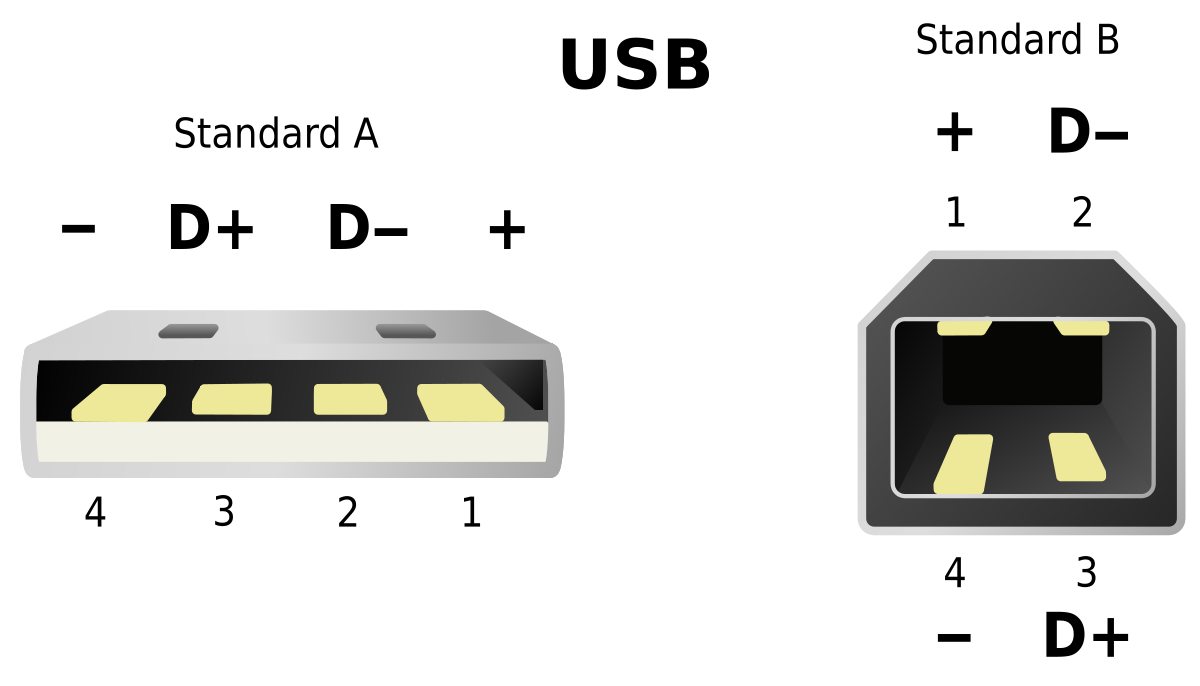
\includegraphics[width=0.7\linewidth]{./Figs/usb_conn.png}
	\caption{\ac{USB} 1.x \& 2.x Connector.}
	\label{fig:usb_conn}
\end{figure}

As illustrated in Figure~\ref{fig:usb_conn}, the original \ac{USB} 1.x \& 2.x
connector only has two pins for data transferring \mbox{(D+ \& D-)}, which has
significantly limited data transfer rate \mbox{(5 Gbits/s Max)} and cannot support
peripherals like DisplayPort \mbox{(10.8 Gbit/s Min)}. Apart from that, support for
other peripherals also requires dedicated transferring lanes as their standards
are not compatible with \ac{USB} in most cases.  

\begin{figure}[t] 
	\centering
	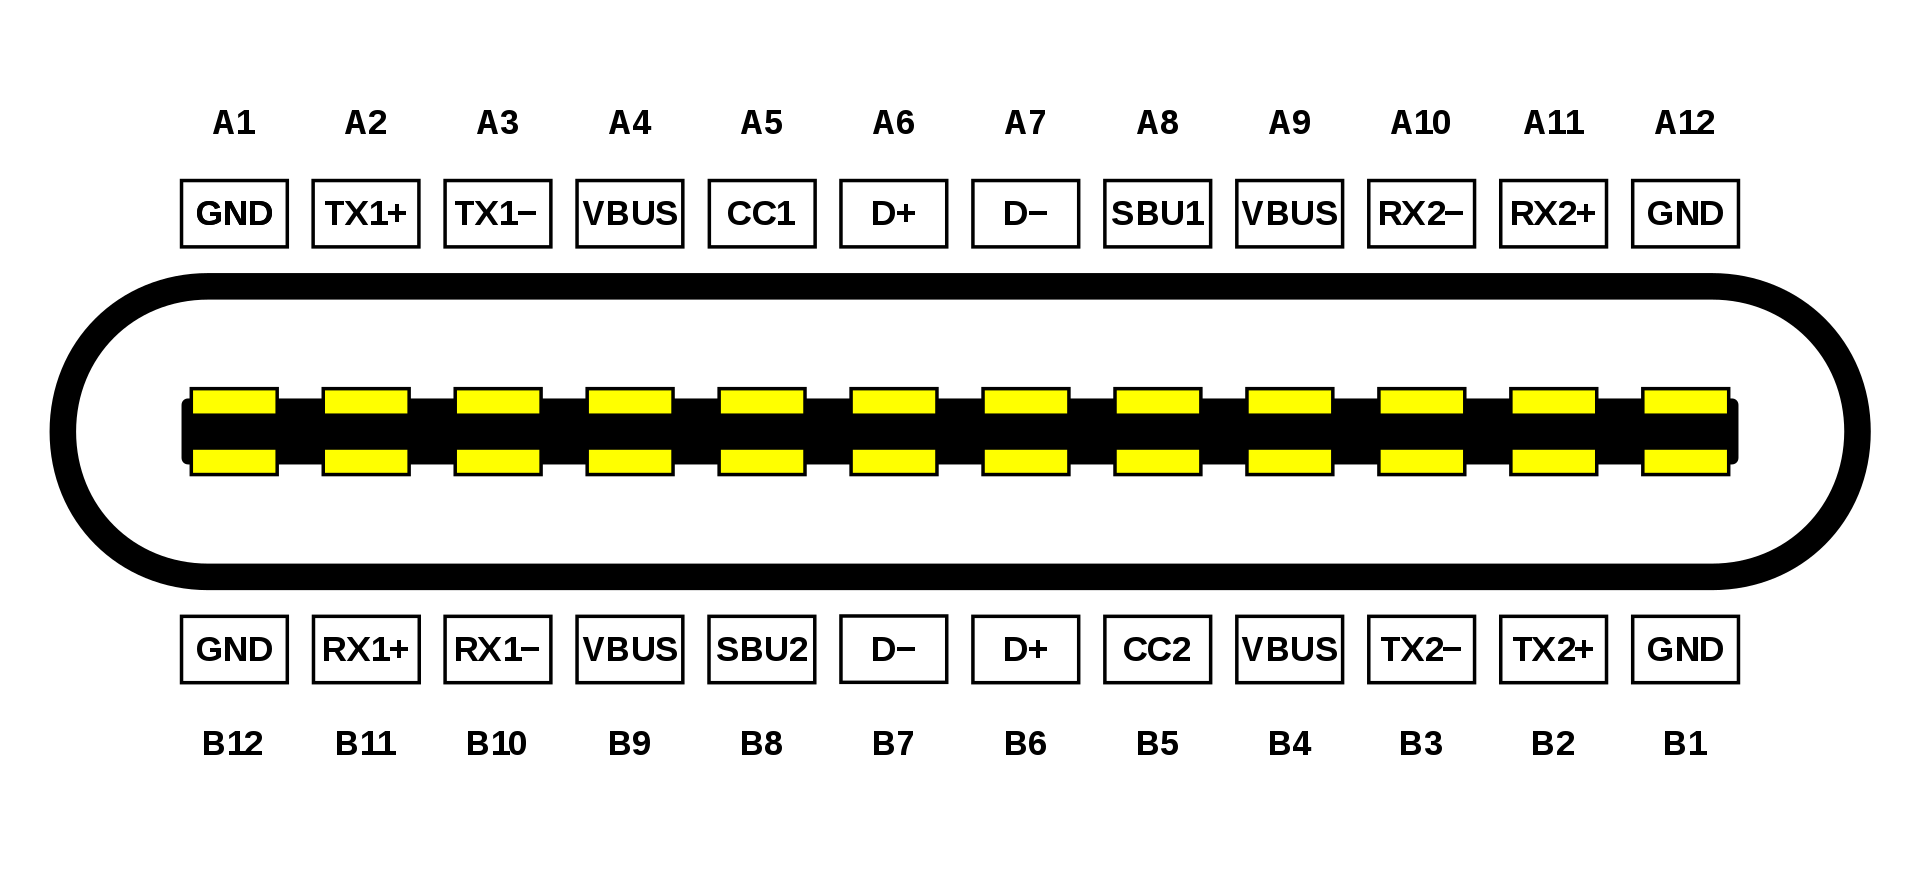
\includegraphics[width=\linewidth]{./Figs/usb_c_conn.png} 
	\caption{\ac{USB} Type-C Connector.} 
	\label{fig:usb_c_conn} 
\end{figure}

Thus, to provide support towards a wider range of peripherals, a 24-pins
standard called \ac{USB} Type-C~\cite{typec} was introduced in 2013 by \ac{USB}-IF~\cite{usbif}. As it is designed to be double-sided, the number of actually usable
pins is halved. Nevertheless, this standard has largely enhanced the capability
of the \ac{USB} 3.x protocol. As presented in Figure~\ref{fig:usb_c_conn}, Type-C added
two high-speed data lanes \mbox{(TRX1 \& TRX2)} and kept the original data lane \mbox{(D+ \&
D-)}. The added lanes are used exclusively to support peripherals like
DisplayPort while the kept data lane transfers \ac{USB} packets.

%\noindent\outline{Security Problem}\\
During the development of \DIFaddbegin \DIFadd{the }\DIFaddend \ac{USB} specification, security was insufficiently considered~\cite{sok}. 
The \ac{USB}-IF believes it is the duty of \acp{OEM}
to decide whether security features should be implemented~\cite{usbsec}. But the divergent implementations give a chance for attacks like
BadUSB~\cite{rubber} and our \tool.

%\fengwei{FIXME: add a reference for each attack in the Table.}
%\fengwei{FIXME: The table is too wide, exceeds the max size.}
\begin{table*}
\begin{tabular}{|c|l|c|c|c|}
	\hline
	\textbf{Year} & \textbf{Protocol Version} & \textbf{Supported Peripherals} & \textbf{Transfer Speed} & \textbf{Attacks} \\
	\hline
	1996 & \ac{USB} 1.x~\cite{usb10,usb11} & Keyboard, Mouse... & 1.5 Mbit/s or 12 Mbit/s & \ac{HID} Emulation (BadUSB)~\cite{badusb} \\
	\hline
	2000 & \ac{USB} 2.0~\cite{usb20} & Flash Drive, High-Definition Link, CD Driver... & 480 Mbit/s & Autorun Attack~\cite{duqu}, Juice Filming~\cite{JFC,JFCImpact} \\
	\hline
	2008 & \ac{USB} 3.0~\cite{usb30} & / & 5 Gbit/s & / \\
	\hline
	2013 & \ac{USB} 3.1~\cite{usb31} & HDMI, DisplayPort, ThunderBolt... & 10 Gbit/s & \tool \\
	\hline
	2017 & \ac{USB} 3.2~\cite{usb32} & / & 20 Gbit/s & / \\
	\hline
\end{tabular}
	\linebreak
\caption{\ac{USB} Protocol Timeline.}
\label{table:usb_timeline}
\end{table*}

\section{Related Work}
\label{sec:related_work}
%\hongyi{Move the stuff about USB protocol to Background}\\
%\outline{Attack based on USB 1.0, briefly}\\
%\outline{Attack based on USB 2.0, focus on works about application and transport layer}\\
%\outline{Attack survey table}\\
%\outline{Attack or current works about USB Type-C}\\

We \DIFdelbegin \DIFdel{survey }\DIFdelend \DIFaddbegin \DIFadd{surveyed }\DIFaddend related works on \ac{USB} attacks in Section~\ref{subsec:usb_attack} and
\ac{USB} security defense in Section~\ref{subsec:usb_defence}, respectively.

\subsection{USB Attacks}
\label{subsec:usb_attack}
%\fengwei{Related work section needs to be improved. Many typos and grammar mistakes can be found.}

During the development of the \ac{USB} protocol, many \mbox{\ac{USB}-based} attacks were proposed,
ranging from \ac{DoS} to protocol masquerading.

%Attacks against USB kernel drivers 
From the kernel perspective, its \ac{USB} software stack generally expects devices
to follow the \ac{USB} standard and may not consider corner cases of malformed \ac{USB}
packets. Based on this, Facedancer~\cite{facedancer} and
Syzkaller~\cite{syzkaller} use fuzzing techniques to uncover the bugs lying in
the kernel drivers. These bugs can cause kernel crashes and lead to a \ac{DoS} attack.
Though this poses a great challenge to the availability of a system, this
attack still requires physical access to the host and is unable to cause more
damage other than \ac{DoS}.

% USB protocol attacks
In the field of \ac{USB} security, protocol masquerading is also a widely used
attack scheme. Due to the lack of authentication in the \ac{USB} protocol, malicious
devices can hide their real functionality with re-written
firmware~\cite{rubber,badusb,rubberducky2020,usbbypassing,iseeyou,usbdriver}.
These works rewrite the firmware of a normal-looking flash drive, which allows
it to act like other devices. When these modified drives are connected to the
host, they could be recognized as a keyboard or mouse. Then the attacker can
execute malicious payloads as they \DIFdelbegin \DIFdel{were }\DIFdelend \DIFaddbegin \DIFadd{are }\DIFaddend using the victim's \DIFdelbegin \DIFdel{devices}\DIFdelend \DIFaddbegin \DIFadd{device}\DIFaddend . Due to the
limitation of \ac{USB} 2.0~\cite{usb20} protocol, these BadUSB
attacks~\cite{badusb} are unable to obtain video feedback from the victim
as video stream was not supported until \ac{USB} 3.0~\cite{usb30}. 
\DIFdelbegin \DIFdel{Although }%DIFDELCMD < \ac{USB} %%%
\DIFdel{2.0 does not
support video transmission, there exists a protocol called }\DIFdelend \DIFaddbegin 

\DIFaddend \ac{MHL} \DIFdelbegin \DIFdel{which }\DIFdelend extends the \ac{USB} standard and allows the video signal to
be transmitted through the \ac{USB} interface \DIFdelbegin \DIFdel{. JFA}\DIFdelend \DIFaddbegin \DIFadd{even for }\ac{USB} \DIFadd{2.0 protocol. 
}\ac{JFA}\DIFaddend ~\cite{JFC},
\DIFdelbegin \DIFdel{short for Juice Filming Attacks is an example that }\DIFdelend abuses this standard and \DIFaddbegin \DIFadd{monitoring the victim's device utilizing }\ac{USB} \DIFadd{2.0 protocol. Although }\ac{JFA}\DIFadd{~\mbox{%DIFAUXCMD
\cite{JFC} }\hspace{0pt}%DIFAUXCMD
could }\DIFaddend exfiltrates video data from the victim\DIFdelbegin \DIFdel{without permission. However, in JFA, this data exfiltration is not
combined with BadUSB attacks, and }\DIFdelend \DIFaddbegin \DIFadd{'s device without permission,  
there are two main limitation compared with }\tool\DIFadd{: 
}\ding{182} \ac{JFA}\DIFadd{~\mbox{%DIFAUXCMD
\cite{JFC} }\hspace{0pt}%DIFAUXCMD
can only exfiltrate video data passively from the victim's device, while }\tool \DIFadd{can control the victim's device at the same time as monitoring the screen. All data can be collected by }\ac{JFA} \DIFadd{only after the victim's interaction, while }\tool \DIFadd{can gather sensitive data actively through }\ac{HID} \DIFadd{injection. For example, if a victim leaves his/her phone charging without locking it, }\ac{JFA} \DIFadd{cannot obtain anything in this case, while }\tool \DIFadd{can actively control his/her device and gather sensitive information.
}\ding{183} \DIFadd{The official list of }\DIFaddend \ac{MHL} \DIFdelbegin \DIFdel{is an outdated standard, which limits its
capability. }\DIFdelend \DIFaddbegin \DIFadd{Devices~\mbox{%DIFAUXCMD
\cite{MHLlist} }\hspace{0pt}%DIFAUXCMD
shows that the latest mobile devices supporting }\ac{MHL} \DIFadd{were released in 2015, which indicates the lack of support of }\ac{MHL} \DIFadd{and limits the attack range of }\ac{JFA}\DIFadd{. }\tool \DIFadd{attacks over }\ac{USB} \DIFadd{Type-C interface, the latest }\ac{USB} \DIFadd{connector designed to replace all previous USB connector including MicroUSB~\mbox{%DIFAUXCMD
\cite{li2018usb}}\hspace{0pt}%DIFAUXCMD
. So }\tool \DIFadd{has a wider attack range. 
}\DIFaddend 

% Using USB devices to inject code
Besides attacking from the protocol perspective, previous works\shuqing{re?} \DIFdelbegin \DIFdel{used }\DIFdelend \DIFaddbegin \DIFadd{use }\DIFaddend a
\ac{USB} device as a payload delivery means. Duqu~\cite{duqu} uses a user-mode
rootkit to hide malicious files on the \ac{USB} storage device, Flame\cite{flame} uses a
zero-day exploit and malicious \textit{autorun.inf} to execute the malware
automatically. There are also works \cite{brain,stuxnet,conficker}
following the same paradigm and performing code-injection attacks. These
attacks are much more damaging and flexible,
but they require certain existing flaws like a zero-day vulnerability\cite{zero-day}  and \ac{USB} is merely
a payload delivery method.

% Using USB for information leakage
As a data transmission protocol, \ac{USB} inevitably leaks electromagnetic signals
to the environment which may contain sensitive information. Leveraging this
physical phenomenon, previous works~\cite{smartphone,
poweremi,revealing,su2017usb,usbgpslocator,bates2014leveraging,badusbhub,usbfinger,side,usbdriver}
eavesdrop on the leaked signals and recover the sensitive data. In a similar fashion, USBee\cite{usbee} and TURNIPSCHOOL\cite{turnip} emit electromagnetic emissions by data injection on the bus
with the connected \ac{USB} devices as an RF transmitter and USBKiller\cite{usbkiller}
\DIFdelbegin \DIFdel{inject }\DIFdelend \DIFaddbegin \DIFadd{injects }\DIFaddend analog
power to cause physical damage to the host machine. Even though the data,
including the video data, could be recovered in this way, these attacks for
executing malicious code are too difficult to work, and invisibility is a
problem that cannot be ignored due to the spatial locality of radio frequency.

Since \ac{USB} 3.1~\cite{usb31} was introduced with \ac{USB} Type-C in 2013, DisplayPort and HDMI
connectors have been provided by \ac{USB} Type-C, transferring of video data can be
combined with the other attacks, like protocol masquerading,  protocol
corruption, and code injection. This has paved the path for our \tool.

\DIFdelbegin \DIFdel{It is worth noting that our }%DIFDELCMD < \tool %%%
\DIFdel{is different from JFA~\mbox{%DIFAUXCMD
\cite{JFC}}\hspace{0pt}%DIFAUXCMD
. Juice Filming Attacks cannot control the attacked device, it can only video-capture user inputs during charging. However, our }%DIFDELCMD < \tool %%%
\DIFdel{can control the attacked device at the same time as monitoring the screen, which enhances the efficiency of stealing users' private data. 
}%DIFDELCMD < 

%DIFDELCMD < %%%
\DIFdelend \subsection{USB Security Defenses}
\label{subsec:usb_defence}

Many defenses have been proposed to defend against BadUSB attacks~\cite{sok}.

From the hardware perspective, the BadUSB attack requires \mbox{\DIFdelbegin \DIFdel{`D-' and `}\DIFdelend \DIFaddbegin \DIFadd{(}\DIFaddend D+ \DIFdelbegin \DIFdel{'}\DIFdelend \DIFaddbegin \DIFadd{\& D-)}\DIFaddend } pins which
are defined by the protocol to transmit data. Without these pins, data cannot 
be transferred via a \ac{USB} cable. Based
on this fact, \ac{USB} Condom~\cite{Condom} is a hardware solution to block data
channels by adding a blocker in the connector. This blocker can cut off the \mbox{\DIFdelbegin \DIFdel{`D-' and `}\DIFdelend \DIFaddbegin \DIFadd{(}\DIFaddend D+ \DIFdelbegin \DIFdel{'}\DIFdelend \DIFaddbegin \DIFadd{\& D-)}\DIFaddend } connection while leaving the power pins intact. However, this method poses
a great challenge to the \ac{PnP} property of \ac{USB}, as once it is deployed, it
stops all \ac{USB} functions other than charging.

Under the premise of ensuring the full functionality of \ac{USB} devices, some works
improve the security while establishing connection. Windows Defender
ATP~\cite{windenfenderwhite} maintains a whitelist of \ac{USB} devices, only devices
on the whitelist are allowed to communicate with the host. This prevents all
potential attacks from untrusted devices, however, this requires users to have a
certain security awareness and technical background to maintain a valid
whitelist. For example, a naive user may add the \ac{USB} device from unknown
sources to his/her whitelist without precaution. Fortunately, some designs have been proposed to overcome
this drawback. For instance, Mohammadmoradi \emph{et al.}~\cite{mohammadmoradi2018making}\shuqing{check name} propose a strategy to generate such a
whitelist automatically. This strategy first generates a unique fingerprint for
each device based on its functionality. Then these fingerprints are used to
maintain a secure and valid whitelist of \ac{USB} devices. There is another work
mediating \ac{USB} connectivity for industrial control. TMSUI~\cite{yang2015tmsui}
relies on the rich experience of administrators to build a whitelist. However, some
modified \ac{USB} devices may hide their real functionality from the user.

To solve this flaw, GoodUSB~\cite{tian2015defending} reports the functionality claimed
by the device to the user and \DIFdelbegin \DIFdel{let }\DIFdelend \DIFaddbegin \DIFadd{lets }\DIFaddend the user decide whether to authorize. When a device
is plugged in, GoodUSB blocks its functionality before enumeration until a
series of authorizations are completed. These authorizations are designed to be
performed manually, thus the malicious devices will be detected if they make a different claim 
that does not match the authorization results. 
USBeSafe\cite{usbesafe} analyses the 
feature vector constructed with the data collected from \DIFdelbegin %DIFDELCMD < \acp{URB}%%%
\DIFdelend \DIFaddbegin \DIFadd{USB Request Blocks}\DIFaddend , 
detects the novel \ac{USB} packets based on the machine learning algorithm and sends 
an alert to the user before enumeration. As BadUSB attacks normally request privileged 
interfaces during enumerating, these defenses are sufficient for these attacks.
Moreover, Mueller \emph{et al.}~\cite{MuellerZN19} improve the security without changing user experience. It can detect the presence of the user, block malicious devices in the user's absence until the session is unlocked.


After the \ac{USB} enumeration and driver loading, some related works follow the \textit{defense in depth} approach to defend against BadUSB attacks.  
Neuner \emph{et al.}~\cite{neuner2018usblock}
prevent BadUSB attacks from the malicious flash drive by analyzing
the temporal characteristics of BadUSB-like attacks. This defense mechanism is
effective because the attacker cannot obtain the screen of the \DIFaddbegin \DIFadd{victim }\DIFaddend host using
BadUSB. In this case, the malicious device can only inject keystrokes in a very
short time to reduce the risk of being discovered. 
This \DIFdelbegin \DIFdel{defect }\DIFdelend \DIFaddbegin \DIFadd{property }\DIFaddend causes the
typing characteristics of BadUSB to be detectable. Pham \emph{et al.}~\cite{pham2010optimizing} optimize Windows security features, which can
block the execution of unsigned files and the installation of unsigned drivers
carried on portable media. Moreover, in GoodUSB, a VM is deployed in the host as
a honeypot to detect and stop malicious behavior of \ac{USB} devices.

In addition to injection attacks, data theft attack is also one of the focuses
of the academic community. As mentioned in Section~\ref{subsec:usb_attack}, there
exists an attack called \DIFdelbegin \DIFdel{JFA}\DIFdelend \DIFaddbegin \ac{JFA}\DIFaddend ~\cite{JFC} which abuses the \ac{MHL}
standard to steal \DIFaddbegin \DIFadd{the }\DIFaddend video stream from the victim. In order to mitigate this
issue, Meng et al.~\cite{meng2018252} propose a statistical model using status
like GPU/CPU usage to detect \DIFdelbegin \DIFdel{JFA }\DIFdelend \DIFaddbegin \ac{JFA} \DIFaddend attacks.

Therefore, there exists a clear trade-off between the effectiveness and the
\ac{PnP} property. Although hardware disabling solutions like \ac{USB} Condom
achieves almost absolute security, the functionality of \ac{USB} is sacrificed.
Other solutions like whitelist are either bypassable or insufficient
under certain scenarios. Vendors may sacrifice complete security to
improve usability, which allows attackers to take advantage of.

We summarize the former efforts on \ac{USB} attacks and defenses in
Table~\ref{table:attack_vs_defense}. \cite{usbkiller, cable,smartphone, poweremi,revealing,su2017usb, usbgpslocator, bates2014leveraging, badusbhub, usbfinger, side, usbdriver, usbee, turnip} are not included in this table, because these works are all recovering or injecting signal on the physical layer, we only illustrate the effectiveness of 
each defense against various attacks, including our \tool, on the software layer in Table~\ref{table:attack_vs_defense}. 

\newcommand{\circlefull}{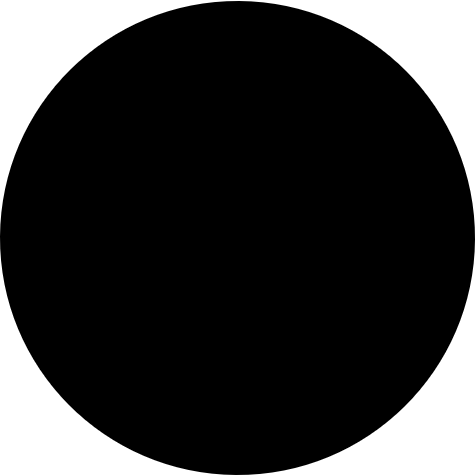
\includegraphics[scale=0.025]{Figs/circle_full.png}}
\newcommand{\circlehalf}{
\includegraphics[scale=0.025]{Figs/circle_half.png}}
\newcommand{\circleempty}{
\includegraphics[scale=0.025]{Figs/circle_empty.png}}
\begin{table*}
	\centering
	\begin{tabular}{|c|c|c|c|c|c|}

		\hline
		\diagbox[width=1.52in,height=0.4in] {\textbf{Defense}}{\textbf{Attack}} & \makecell*[c]{Facedancer~\cite{facedancer},\\ Syzkaller~\cite{syzkaller}} &\cite{rubber, badusb, rubberducky2020, usbbypassing, iseeyou, usbdriver} & JFC~\cite{JFC}&		\makecell{
			Duqu~\cite{duqu}, \\
			\cite{brain, stuxnet, conficker,flame}} & \tool \\
		\hline
		\makecell{\ac{USB} condom~\cite{Condom}} & \makecell*[c]{\circlefull} & \circlefull & \circlefull &\circlefull& \circlefull\\
		\hline
		\makecell{
			Windows Defender ATP~\cite{windenfenderwhite}, \\
			Mohammadmoradi \emph{et al.}~\cite{mohammadmoradi2018making}, \\
			TMSUI~\cite{yang2015tmsui}
		}& \circleempty & \circlehalf & \circlehalf &\circlehalf& \circlehalf\\

		\hline
		\makecell{GoodUSB~\cite{tian2015defending}} & \makecell*[c]{\circlehalf} & \circlefull & \circlefull &\circlefull& \circlefull\\
		\hline

		\makecell{USBeSafe~\cite{usbesafe}} & \makecell*[c]{\circleempty} & \circlefull & \circlefull &\circlefull& \circlefull\\
		\hline

		\makecell{Mueller \emph{et al.}~\cite{MuellerZN19}} & \makecell*[c]{\circleempty} & \circlefull & \circlefull &\circlehalf& \circlefull\\
		\hline

	

		\makecell{Neuner \emph{et al.}~\cite{neuner2018usblock}} & \makecell*[c]{\circleempty} & \circlefull & \circleempty &\circleempty& \circleempty\\
		\hline
		\makecell{Pham \emph{et al.}~\cite{pham2010optimizing}} & \makecell*[c]{\circleempty} & \circleempty & \circleempty &\circlefull& \circleempty\\
		\hline
		\makecell{JFCGuard~\cite{meng2018252}} & \makecell*[c]{\circleempty} & \circleempty & \circlehalf &\circleempty&   \circlehalf \\
			\hline
	\end{tabular}
	\linebreak
    \begin{tablenotes}
	\footnotesize
	\item[1] \circlefull  \@ means that the defense is effective
	\item[2] \circlehalf \@ means that the defense is partial effective
	\item[3] \circleempty \@  means that the defense is not effective
	\end{tablenotes}
	\caption{Effectiveness of Defenses against \ac{USB} Attacks}
	\label{table:attack_vs_defense}
\end{table*}





\section{\tool}
\label{sec:badusb}
\subsection{Threat Model}

We build our threat model on a basic assumption that common users without
technical background would not treat a normal-looking \ac{USB} device as malicious and be cautious about them. This assumption is consistent with existing works~\cite{JFCImpact}. Moreover, we omit the
effect of notifications from \ac{USB} devices, as users may not have the knowledge to fully understand such notifications.

We also assume the victim's device is equipped with fully functional \ac{USB} 3.x
protocol and \ac{USB} Type-C connector. As the \ac{USB} 3.x standard is
common nowadays, this assumption can be fulfilled in recent
devices.

%\subsection{Motivation}
%\noindent\outline{Limitation of Rubber Ducky}\\
%\outline{Our functionality different mode listing?}\\
%\hongyi{The following mode is to be further decided}
%\outline{Automatic Scripting Mode}\\
%\outline{Remote Control Mode}\\
%\outline{OCR/QR Recognition Mode}\\

\subsection{Implementation}
%\noindent\hongyi{The following mode is to be further decided}\\
%\outline{DETAIL of each mode}\\ \outline{Automatic Scripting Mode}\\
%\outline{Remote Control Mode}\\ \outline{OCR/QR Recognition Mode}\\

As introduced in Section~\ref{sec:related_work},
existing works~\cite{rubber,badusb,
rubberducky2020,usbbypassing,iseeyou,usbdriver} focus on BadUSB attacks.
Many of these take advantage of the \textit{trust-by-default} policy of PC,
pretend to be normal \ac{HID} devices and utilize \DIFaddbegin \DIFadd{the }\DIFaddend \ac{USB} protocol to perform attacks.
However, these attacks suffer from various drawbacks: \ding{182} attackers can
only simulate limited types of devices such as \acp{HID} (e.g. keyboards and mice)
and disks, which makes the attacks less effective; \ding{183} accurate attacks
could not be performed due to \DIFaddbegin \DIFadd{a }\DIFaddend lack of \ac{UI} status. Whatever \acp{HID} the
attackers simulate their \ac{USB} devices to be, they could not obtain the \ac{UI} to
check the status information, which makes it nearly impossible to carry out
their attacks precisely or know the effects after attacks.

%Though BadUSB devices\cite{badusb} like Rubber Ducky\cite{rubber,
%rubberducky2020} emulates as a HID device enabling various arbitrary execution
%attacks, fetching feedback from the victim is much more limited.
Based on the drawbacks introduced above, several defense mechanisms were
proposed. For example, GoodUSB~\cite{tian2015defending}
implemented an authorization procedure when a new device is plugged in and blocks other functions except authorized ones.

In this work, we utilize the new features of \ac{USB} 3.x~\cite{usb31,usb32} to
address the problems above.  Benefiting from the latest protocol, we simulate
an external display and thus obtain the video stream to perform accurate
attacks. However, we \DIFaddbegin \DIFadd{are }\DIFaddend still unable to bypass defenses like GoodUSB~\cite{tian2015defending}, which completely blocks unauthorized functionality. This will be further discussed in Section~\ref{sec:discussion}

As there were various BadUSB implementations available, this work focuses on our new extensions. Next, we first introduce the
components we used in \tool, then we focus on the three different attack modes
we implement for various scenarios.

\subsubsection{Attack Model}

Figure~\ref{fig:attack_model} shows the architecture of our attack model. \circled[text=white,fill=myyellow]{\footnotesize{1}} represents the victim's devices; \circled[text=white,fill=myyellow]{\footnotesize{2}} is our \tool; \circled[text=white,fill=myyellow]{\footnotesize{3}} is the attacker's remote PC. The details of each component in \tool are as follows.

%\fengwei{We need to
%explain the figure. What are the boxes? Where is victim? Where is the attacker?
%The list below only shows the internal components in the malicious \ac{USB} device.
%We might also consider to explain this in the Figure caption.}

\begin{itemize}

	\item\underline{USB 3.x Hub} exports the \ac{USB} 3.x connector into various ports, like DisplayPort, \ac{USB} 2.0 port, etc.

	\item\underline{Video Capture Card} converts DisplayPort signal into compatible data, which is later processed by the Single Board Computer (i.e., an embedded computer).

	\item\underline{\ac{HID} Emulator} emulates \ac{HID} device which can be controlled by the attacker.

	\item\underline{Single Board Computer} processes \DIFaddbegin \DIFadd{the }\DIFaddend video stream from the victim via the Video Capture Card or sends commands to the victim via \ac{HID} Emulator.

	\item\underline{Wi-Fi/GSM Module} transmits the sensitive data or receives commands to/from the remote attacker PC.

\end{itemize}


\begin{figure}[t]
	\centering
	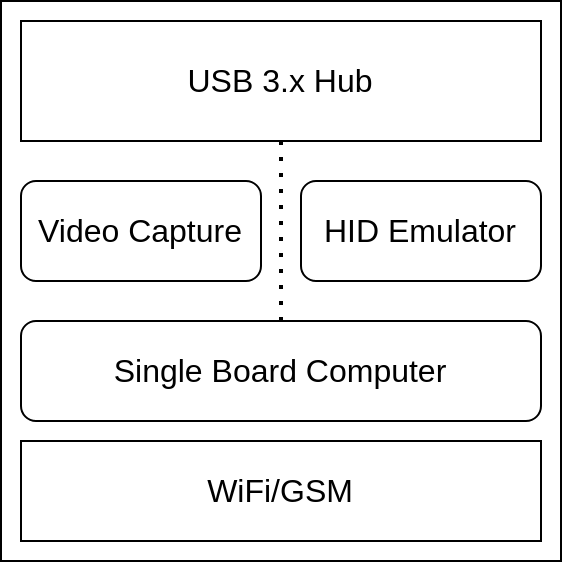
\includegraphics[width=\linewidth]{./Figs/attack_model.png}

	\begin{tabular}{ll}
	\circled[text=white,fill=myyellow]{\footnotesize{1}} Victim's Devices    &\circled[text=white,fill=myyellow]{\footnotesize{2}}~\tool\\
	\circled[text=white,fill=myyellow]{\footnotesize{3}} Attacker's Remote PC
	\end{tabular}

	\caption{Attack Model.}%\shuqing{Need to be more compact.}
	\label{fig:attack_model}
\end{figure}

\textbf{\ac{HID} Emulation Mode.} This mode mainly relies on the ``\ac{HID} Emulator'' in Figure~\ref{fig:attack_model} to
send constructed \ac{HID} \DIFdelbegin \DIFdel{packet }\DIFdelend \DIFaddbegin \DIFadd{packets }\DIFaddend to the victim. These constructed \ac{HID} packets are
interpreted by the victim as valid keystrokes and mouse \DIFdelbegin \DIFdel{moves}\DIFdelend \DIFaddbegin \DIFadd{movements}\DIFaddend . Thus, \DIFdelbegin \DIFdel{the
attacker }\DIFdelend \DIFaddbegin \DIFadd{attackers }\DIFaddend can execute arbitrary scripts on the victim's device. This is the
function of \DIFdelbegin \DIFdel{the original }\DIFdelend BadUSB. Based on this, we made the following
improvements.

First, as \tool has established a feedback channel using \ac{USB} \DIFdelbegin \DIFdel{3.2 }\DIFdelend \DIFaddbegin \DIFadd{3.x }\DIFaddend protocol, when performing keystroke and mouse \DIFdelbegin \DIFdel{movement }\DIFdelend \DIFaddbegin \DIFadd{movements }\DIFaddend injection, an attacker can obtain real-time feedback from the victim's \DIFdelbegin \DIFdel{devices}\DIFdelend \DIFaddbegin \DIFadd{device}\DIFaddend . This feedback allows an attacker to tell whether the previous attack succeeded and decide what to perform next. Existence of such a feedback channel largely strengthens the attack ability of \tool.

Moreover, as the mouse relies on the visual feedback to work properly, its
emulation and automation were not supported by the original version of BadUSB.
Yet with the video output support from \ac{USB} 3.x, our \tool implements a
fully-functional mouse emulation. This function enables attacks toward pure \ac{GUI}
programs and shows potential in the mobile attack scenarios. Details can
be obtained in Section~\ref{sec:experiment}.

The advantage of this mode is that it achieves attack
feedback with video streaming.
%\fengwei{I don't understand the sentence below.}\hongyi{Fixed, I think it's redundant and less important}
%As mentioned above, we only require video stream at the beginning (defense
%bypass) and the end (result feedback) of the attack.
Also, with mouse
supported, \tool extends the original BadUSB attack and results in further attacks\DIFdelbegin \DIFdel{in
mobile devices}\DIFdelend .

\textbf{Video Capture Mode.} \tool under this mode does not emulate other
USB device and solely relies on the video stream function of \ac{USB} 3.x; it uses the
``Video Capture'' component as shown in the Figure~\ref{fig:attack_model} to transmit the stream to the embedded ``Single Board Computer''.
%\fengwei{What is embedded computer? Do we define this in the previous\hongyi{Fixed by using the term mentioned in Figure}
%text?}.
The victim's device mistakenly treats \tool as an external monitor
and output its video stream. This stream is \DIFdelbegin \DIFdel{latter }\DIFdelend \DIFaddbegin \DIFadd{later }\DIFaddend processed by the embedded
computer to extract sensitive data.

When running in this mode, \tool passively processes the victim's video stream
and detects ``valuable'' private data.  The data is considered as
``valuable'' or not by a customized detector. We implemented a simple
payment code detector for the proof-of-concept purpose, which demonstrates that we successfully \DIFdelbegin \DIFdel{transfer }\DIFdelend \DIFaddbegin \DIFadd{transfered }\DIFaddend money from a victim to an
attacker. More detail can be obtained in Section~\ref{sec:experiment}.

It is worth mentioning that \tool under this mode is completely passive, making
it hard to be detected. With different detectors implemented, \tool
under this mode is capable of serving more purposes.

\textbf{Full Control Mode.} In \tool, we have implemented all components
required to control a computer/mobile device completely, including a video stream
and a keyboard/mouse emulation. Thus with all components enabled, not only does
the victim's device treat \tool as an external display, but also a valid \ac{HID}
input source. Hence we can achieve complete hijack of the victim's device.

\tool under this mode follows a simple logic. \tool receives video stream
from the victim's device and redirects it to the attacker via GSM/WiFi. In the
meanwhile, \tool also receives keystrokes and mouse movements from the attacker
through GSM/WiFi and replays them to the victim\DIFaddbegin \DIFadd{'s device }\DIFaddend by the \ac{USB} emulation.

This mode enables attackers to perform delicate operations that are beyond
automation. Moreover, this mode provides a backdoor that does not require a host
network and thus is undetectable by the firewall running on the host machine.
%\hongyi{I think this is a quite good selling point?}\shuqing{Agree with
%Hongyi.}

The advantage of this mode is that it can completely hijack the victim's device
and provides a backdoor beyond detection of firewalls; however, this complete control
also comes with the price of high power consumption and risk of being detected
by the user.


\section{Experiment}
\label{sec:experiment}
%\shuqing{Many parts in this section are much more likely to lie in implementation, introducing how \tool works. Doesn't look like experiment.}

%\shuqing{Experiment for devices and case study needed.}

To evaluate the effectiveness of \tool in different modes, we conducted three
experiments on \tool using devices with \ac{USB} Type-C capabilities from different
\acp{OEM}, including a mobile phone, a tablet, and a laptop.

\textbf{Setup.}
%\fengwei{I would suggest to add references for devices such as
%Pi, ATMEGA32U4 board, Yamazawa, etc.}
As mentioned in Section~\ref{sec:badusb},
our \tool only requires common components that are easily accessible online or
in any electronic store. Here we \DIFdelbegin \DIFdel{choose }\DIFdelend \DIFaddbegin \DIFadd{chose }\DIFaddend the following parts to build a
prototype. To begin with, we \DIFdelbegin \DIFdel{choose }\DIFdelend \DIFaddbegin \DIFadd{chose }\DIFaddend the Raspberry Pi 4B~\cite{pi4b} as the embedded Single Board
Computer inside \tool, which is powerful enough to process video data and has
an onboard WiFi chip. As for the \ac{HID} Emulator, we \DIFdelbegin \DIFdel{use }\DIFdelend \DIFaddbegin \DIFadd{used }\DIFaddend an Atmel ATMEGA32U4 board~\cite{atmel}
with \ac{USB} protocol support, which is able to emulate multiple \acp{HID}
with our modified firmware. About the \ac{USB} 3.x Hub, we \DIFdelbegin \DIFdel{use one from
the
}\DIFdelend \DIFaddbegin \DIFadd{used one from
}\DIFaddend UGREEN~\cite{ugreen}, which supports HDMI, \ac{USB} 2.0, and many other exported peripherals.
Apart from these essential parts, we also \DIFdelbegin \DIFdel{use }\DIFdelend \DIFaddbegin \DIFadd{used }\DIFaddend an auxiliary power bank to
provide power for the Raspberry Pi and the mobile devices used by the victim.
The image of our \tool prototype can be found in Figure~\ref{fig:armory}.

\circled[text=white,fill=myblue]{\scriptsize{A}} is a \DIFdelbegin \DIFdel{Huawei }\DIFdelend \DIFaddbegin \DIFadd{HUAWEI }\DIFaddend mobile phone, the victim's device; \circled[text=white,fill=myblue]{\scriptsize{B}} is a compact look of \tool prototype; \circled[text=white,fill=myblue]{\scriptsize{1}} is the \ac{USB} 3.x Hub; \circled[text=white,fill=myblue]{\scriptsize{2}} is a Raspberry Pi 4B as the Single Board Computer; \circled[text=white,fill=myblue]{\scriptsize{3}} is an auxiliary power bank; \circled[text=white,fill=myblue]{\scriptsize{4}} is the Video Capture Card; \circled[text=white,fill=myblue]{\scriptsize{5}} is an Atmel ATMEGA32U4 board as the \ac{HID} Emulator.
%\fengwei{We need to explain the Figure. What is "A"? What is "B", Where are 1,
%2, 3, 4, and 5?}\hongyi{Is the caption sufficient? If explain here, I feel quite redundant}
%\fengwei{I think it is necessary to explain them in the text again.}


\begin{figure}[t]
	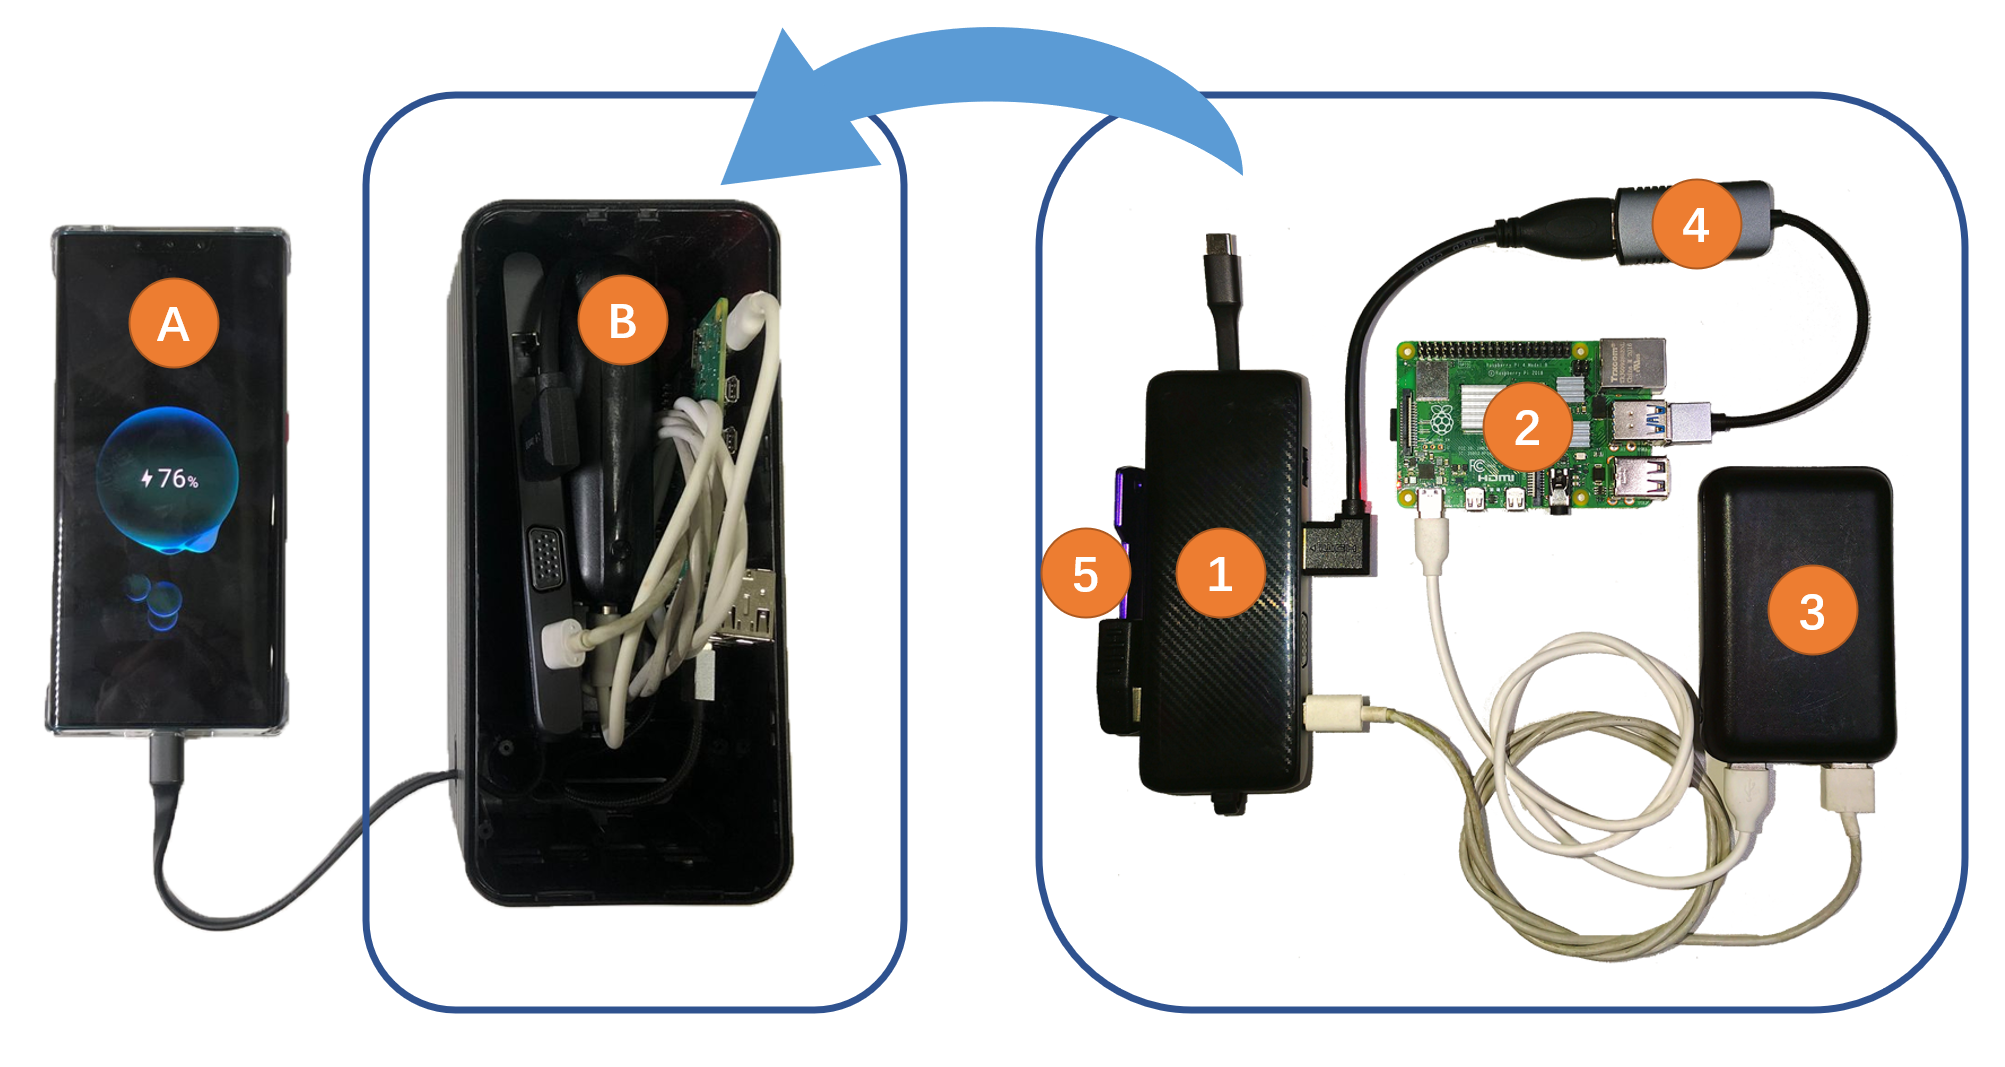
\includegraphics[width=\linewidth]{./Figs/armory_all.png}\\
	\begin{tabular}{ll}
	\circled[text=white,fill=myblue]{\scriptsize{A}} Victim's Device    &\circled[text=white,fill=myblue]{\scriptsize{B}}~\tool\\
	\circled[text=white,fill=myblue]{\footnotesize{1}} \ac{USB} 3.x Hub        &\circled[text=white,fill=myblue]{\footnotesize{2}} Raspberry Pi 4B\\
	\circled[text=white,fill=myblue]{\footnotesize{3}} Auxiliary Power Bank &\circled[text=white,fill=myblue]{\footnotesize{4}} Video Capture\\
	\circled[text=white,fill=myblue]{\footnotesize{5}} ATMEGAA32U4 Board
	\end{tabular}


	\caption{\tool Prototype.}
	\label{fig:armory}
\end{figure}

\subsection{Attack Initialization}
\DIFaddbegin \label{subsec:attack_init}
\DIFaddend After the \tool is plugged into the victim's device, there is an initialization process to make sure the \tool is able to carry out subsequent \DIFdelbegin \DIFdel{attack}\DIFdelend \DIFaddbegin \DIFadd{attacks}\DIFaddend .
\begin{itemize}
	\item \textbf{Screen Mirror}:
		During our experiment, we noticed that some devices \DIFdelbegin \DIFdel{do }\DIFdelend \DIFaddbegin \DIFadd{did }\DIFaddend not mirror their \DIFdelbegin \DIFdel{screen }\DIFdelend \DIFaddbegin \DIFadd{screens }\DIFaddend to our \tool by default. In this case, \tool \DIFdelbegin \DIFdel{will }\DIFdelend \DIFaddbegin \DIFadd{would }\DIFaddend inject a sequence of keystrokes \DIFdelbegin \DIFdel{and mouse movements }\DIFdelend to set the victim's device \DIFdelbegin \DIFdel{into mirror their screen. For example, in }\DIFdelend \DIFaddbegin \DIFadd{to mirror the primary screen. In both }\DIFaddend Windows 10 \DIFaddbegin \DIFadd{and Ubuntu (Gnome Desktop)}\DIFaddend , \tool can inject \DIFdelbegin \DIFdel{`}\DIFdelend \DIFaddbegin \DIFadd{``}\DIFaddend Win+P\DIFdelbegin \DIFdel{' keystroke and a mouse click on the `Duplicate'option. However, as }%DIFDELCMD < \tool %%%
\DIFdel{is unable to obtain the screenduring this process, this can only be performed blindly with a possibility of failure.
		}\DIFdelend \DIFaddbegin \DIFadd{'' (The ``Win'' key is the ``Super'' key in Windows and Ubuntu by default) to switch between different modes for external display. Figure~\ref{fig:ubuntu_switch} illustrates how these keystrokes works on Ubuntu and it is similar in Windows 10. In MacOS, according to the official manual~\mbox{%DIFAUXCMD
\cite{appleman}}\hspace{0pt}%DIFAUXCMD
, }\tool \DIFadd{can inject \mbox{``Command+F1''} keystrokes to set the victim's device to mirror the primary screen. In EMUI, there is a special mode called ``Desktop Mode'', which allows users to use their smartphones like a desktop computer with an external screen. If this mode is enabled, as victim's ``desktop'' can be obtained, }\tool \DIFadd{can inject mouse movements to switch to mirror mode.
		}\begin{figure}[H]
			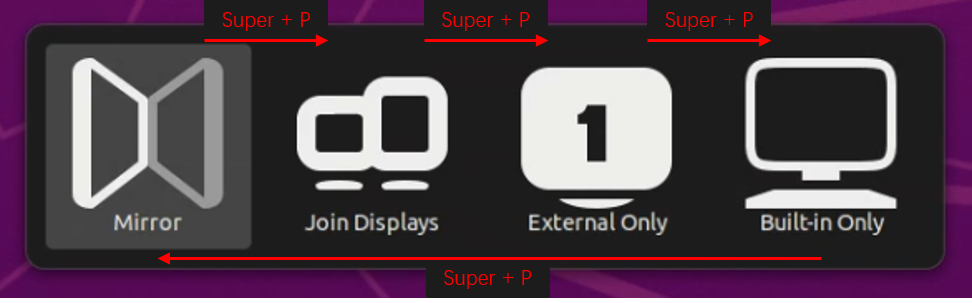
\includegraphics[width=\linewidth]{./Figs/ubuntu_switch.png}\\
			\caption{\DIFaddFL{Switching Screen Mode in Ubuntu.}}
			\label{fig:ubuntu_switch}
		\end{figure}
	\DIFaddend \item \textbf{Dismiss Notification}:
		In our experiment, we found that some devices \DIFdelbegin \DIFdel{will }\DIFdelend \DIFaddbegin \DIFadd{would }\DIFaddend notify the user the presence of an external screen. During our experiment, the following notifications were raised:
		\begin{itemize}
		 \item On Lenovo Xiaoxin Pro 13, it raised a pop-up asking user to select the functionality of the external screen.
		 \item On \DIFdelbegin \DIFdel{Huawei }\DIFdelend \DIFaddbegin \DIFadd{HUAWEI }\DIFaddend P30, it showed a status bar indicator and a persistent notification about the external monitor.
		 \item On iPad Pro (the third generation), it also showed a blue status bar indicator and a notification about \ac{USB} accessories if iPad is locked.
		\end{itemize}
		To avoid being discovered by the victim, \tool can inject keystrokes and mouse movements to dismiss some of these notifications. For example, in the first case, \tool is able to inject a sequence of mouse movements to set the screen at mirror mode to dismiss the pop-up.
\end{itemize}
\begin{comment}
\begin{table*}[]
	\begin{tabular}{|c|c|c|c|}
		\hline
		Device                                                               & Operating System                                                                                         & Notification              & Dismiss Action                                            \\ \hline
		\begin{tabular}[c]{@{}c@{}}Lenovo Xiaoxin Pro 13\\ 2020\end{tabular} & Windows 10 (OS Build 18363.1379)                                                                         & Pop-up                    & ``Win+P''-\textgreater{}Mouse click on `Duplicate' Option \\ \hline
		\multirow{2}{*}{HUAWEI P30 (ELE-AL00)}                               & \multirow{2}{*}{\begin{tabular}[c]{@{}c@{}}EMUI 11.0.0.135(C00E128R2P5)\\ Android 10 based\end{tabular}} & Status bar indicator      & N/A                                                       \\ \cline{3-4}
		&                                                                                                          & Persistent notifications  & N/A                                                       \\ \hline
		\multirow{2}{*}{iPad Pro (3rd generation)}                           & \multirow{2}{*}{iOS 14.4 (Build 18D52)}                                                                  & Status bar indicator      & N/A                                                       \\ \cline{3-4}
		&                                                                                                          & Pop-up (only when locked) & N/A                                                       \\ \hline
	\end{tabular}
	\linebreak
	\caption{Notifications about \tool}
	\label{tab:notification}
\end{table*}
\end{comment}

\subsection{HID Emulator Mode}

In the experiment of HID emulator mode, we used {Lenovo Xiaoxin Pro 13
2020}, a PC \DIFdelbegin \DIFdel{in }\DIFdelend \DIFaddbegin \DIFadd{with }\DIFaddend Windows 10 \mbox{(OS Build 18363.1379)} \DIFaddbegin \DIFadd{and Ubuntu 20.04.2 LTS }\DIFaddend with two \ac{USB} Type-C interfaces as the
target \DIFdelbegin \DIFdel{device}\DIFdelend \DIFaddbegin \DIFadd{devices}\DIFaddend . During this experiment, \tool disguised itself as a normal keyboard and an external screen as feedback channel. When first plugged in, the victim's \DIFdelbegin \DIFdel{devices }\DIFdelend \DIFaddbegin \DIFadd{device }\DIFaddend raised a pop-up window asking \DIFdelbegin \DIFdel{victims what }\DIFdelend \DIFaddbegin \DIFadd{the victim which }\DIFaddend mode should the new screen be set to. \tool immediately injected a sequence of mouse movements and clicks to set itself as a mirror to the primary monitor. Thus we had successfully completed the attack initialization. Then we tested three scripts, ranging from reverse shell backdoor to malware payload execution, all of \DIFdelbegin \DIFdel{which }\DIFdelend \DIFaddbegin \DIFadd{them }\DIFaddend resulted in success. Compared to original BadUSB attacks like Rubber Ducky, our \tool can provide attackers real-time feedback which allows attackers to perform more accurate attacks.
%This also warned us that we need more thorough defense against such BadUSB
%attack.


%\fengwei{do we need a reference for OCR?}
%\hongyi{we have discussed this and decide no need.}
\subsection{Video Capture Mode}

During the experiment of privacy extraction via our video capture mode, we chose \DIFdelbegin \textit{\DIFdel{HUAWEI P30 (ELE-AL00)}}%DIFAUXCMD
\DIFdelend \DIFaddbegin \DIFadd{\mbox{\textit{HUAWEI P30 (ELE-AL00)}}}\DIFaddend , a
smartphone in \DIFdelbegin \DIFdel{EMUI 11.0.0.135(C00E128R2P5) }\DIFdelend \DIFaddbegin \DIFadd{\mbox{EMUI 11.0.0.135(C00E128R2P5)} }\DIFaddend \mbox{(Android 10.0 based)} with a \ac{USB} Type-C interface, as the
target device. In the privacy extraction experiment, \tool passively captured video
from the victim's device and used \textit{OpenCV} to identify the sensitive
information from the video stream.  When the victim viewed text or photos with
text, \tool used the techniques of \ac{OCR}  to
extract text from corresponding video frames. In this experiment, the attacker
successfully extracted text such as name, address, ID number, and other sensitive
personal information. We also tested the payment code extractor, which enables
an attacker to identify payment code in the video stream and performs transactions
without the password. \DIFaddbegin \DIFadd{During our experiment, we noticed that this HUAWEI device supports `Desktop Mode'
for its external screen, which enables user to use their devices like a desktop computer with a external screen.
If }\tool \DIFadd{is set into this mode, }\tool \DIFadd{is able to inject mouse movements to set itself into mirroring the primary screen, as we discussed in Section~\ref{subsec:attack_init}.
}\DIFaddend As this is also a part of our case study, more details about
the extracted sensitive data can be found in Section~\ref{subsec:case_study} and
Table~\ref{table:information_extracted}.

%\fengwei{I don't understand the following sentence. Both modes need to capture
%the video stream. Don't understand why it is more power-efficient.}
%\hongyi{Reasonable, changed to other advantage}
Note that the video capture mode only needs to
process the victim's video stream locally, it does not need to transmit the real-time video back to the attacker, which is useful when the network connection between \tool and the attacker is not stable.
%This mode is useful when there is no stable network connection between \tool and the attacker.

\subsection{Fully Control Mode}
%\fengwei{In BadUSB-C section, remote control model is after privacy extraction mode.}

To test the capability of the full control mode, we chose iPad Pro (3rd
	generation), a tablet \DIFdelbegin \DIFdel{in }\DIFdelend \DIFaddbegin \DIFadd{running }\DIFaddend iOS 14.4 (Build 18D52) with a \ac{USB} Type-C interface, as the target
device in this experiment.  Besides disguising \DIFaddbegin \DIFadd{themself }\DIFaddend as normal \acp{HID} like a
conventional BadUSB~\cite{badusb}, \tool also transmitted real-time video
stream from the target device to the attacker via WiFi.  After establishing the connection, the attacker performed a series of actions to test the capability of
\tool. In the beginning, the attacker accessed the album application on the iPad and
obtained all the photos inside. After that, the attacker sent messages via the victim's
account. At last, the attacker performed a transaction using the
financial application. All of these tests resulted in success.

Through this experiment, we have found that with video transmission and mouse
emulation, \tool extensively expanded the attack capability of BadUSB,
especially in mobile devices. In short, we have achieved the complete hijack of the victim's
device in this experiment.

\subsection{Case study}
\label{subsec:case_study}
\tool can be used in various attack scenarios, ranging from mobile devices to PC devices.
For example, \tool can be attached to the power station, which provides USB 3.x hubs, in the airport to perform attacks.
Most people charge their laptops or smartphones in the power station in emergency, with negligence of security.
In the following paragraphs, we will demonstrate the attack scenarios of \tool using sharing power bank as an example.

\subsubsection{Background}

\DIFdelbegin %DIFDELCMD < \begin{table*}[t]
%DIFDELCMD < 	\centering
%DIFDELCMD < 	\begin{tabular}{|l|l|l|l|}
%DIFDELCMD < 		\hline
%DIFDELCMD < 		%%%
\textbf{\DIFdelFL{Keyword}} %DIFAUXCMD
%DIFDELCMD < & %%%
\textbf{\DIFdelFL{Text}}                                                             %DIFAUXCMD
%DIFDELCMD < & %%%
\textbf{\DIFdelFL{Name}}                                   %DIFAUXCMD
%DIFDELCMD < & %%%
\textbf{\DIFdelFL{Frame Number}} %DIFAUXCMD
%DIFDELCMD < \\ \hline
%DIFDELCMD < 		%%%
\DIFdelFL{username                          }%DIFDELCMD < & %%%
\DIFdelFL{X 8B cas.******.edu.cn Username: 11****18 Password:                                        }%DIFDELCMD < & %%%
\DIFdelFL{\textless{}user1\textgreater{} }%DIFDELCMD < & %%%
\DIFdelFL{385                                    }%DIFDELCMD < \\ \hline
%DIFDELCMD < 		%%%
\DIFdelFL{username                          }%DIFDELCMD < & %%%
\DIFdelFL{Login Weibo Login with SMS and verification code ...... +86 151****4587                    }%DIFDELCMD < & %%%
\DIFdelFL{\textless{}user5\textgreater{} }%DIFDELCMD < & %%%
\DIFdelFL{1947                                   }%DIFDELCMD < \\ \hline
%DIFDELCMD < 		%%%
\DIFdelFL{username                          }%DIFDELCMD < & %%%
\DIFdelFL{QQ 14*****50| Login with phone number New user registration 2345678 9 0                    }%DIFDELCMD < & %%%
\DIFdelFL{\textless{}user3\textgreater{} }%DIFDELCMD < & %%%
\DIFdelFL{4308                                   }%DIFDELCMD < \\ \hline
%DIFDELCMD < 		%%%
\DIFdelFL{username                          }%DIFDELCMD < & %%%
\DIFdelFL{connect to *** username h*****l Save account information Open VPN.....                     }%DIFDELCMD < & %%%
\DIFdelFL{\textless{}user6\textgreater{} }%DIFDELCMD < & %%%
\DIFdelFL{7925                                   }%DIFDELCMD < \\ \hline
%DIFDELCMD < 		%%%
\DIFdelFL{phone number                      }%DIFDELCMD < & %%%
\DIFdelFL{Login with phone number ...... +86 186****2483 |                                           }%DIFDELCMD < & %%%
\DIFdelFL{\textless{}user1\textgreater{} }%DIFDELCMD < & %%%
\DIFdelFL{313                                    }%DIFDELCMD < \\ \hline
%DIFDELCMD < 		%%%
\DIFdelFL{phone number                      }%DIFDELCMD < & %%%
\DIFdelFL{Log in with your mobile phone number. ...... mobile phone number 131****9310 }%DIFDELCMD < & %%%
\DIFdelFL{\textless{}user9\textgreater{} }%DIFDELCMD < & %%%
\DIFdelFL{210                                    }%DIFDELCMD < \\ \hline
%DIFDELCMD < 		%%%
\DIFdelFL{@                                 }%DIFDELCMD < & %%%
\DIFdelFL{contact email 30*******7G@qq.com, contact phone 027-88******                               }%DIFDELCMD < & %%%
\DIFdelFL{\textless{}user7\textgreater{} }%DIFDELCMD < & %%%
\DIFdelFL{5324                                   }%DIFDELCMD < \\ \hline
%DIFDELCMD < 		%%%
\DIFdelFL{@                                 }%DIFDELCMD < & %%%
\DIFdelFL{Account 73*****5@qq.com @qq.com @163.com @gmail.com 	......      }%DIFDELCMD < & %%%
\DIFdelFL{\textless{}user6\textgreater{} }%DIFDELCMD < & %%%
\DIFdelFL{621                                    }%DIFDELCMD < \\ \hline
%DIFDELCMD < 	\end{tabular}
%DIFDELCMD < 	\linebreak
%DIFDELCMD < 	%%%
%DIFDELCMD < \caption{%
{%DIFAUXCMD
\DIFdelFL{Examples of Searching }%DIFDELCMD < \ac{OCR} %%%
\DIFdelFL{Results with Keywords.}}
	%DIFAUXCMD
%DIFDELCMD < \label{tab:ocr_keyword_example}
%DIFDELCMD < \end{table*}
%DIFDELCMD < 

%DIFDELCMD < \begin{table*}[t]
%DIFDELCMD < 	\centering
%DIFDELCMD < 	\begin{tabular}{|c|c|c|c|c|c|c|}
%DIFDELCMD < 		\hline
%DIFDELCMD < 		%%%
\textbf{\DIFdelFL{Keyword}}                               %DIFAUXCMD
%DIFDELCMD < & %%%
\DIFdelFL{Account }%DIFDELCMD < & %%%
\DIFdelFL{Password }%DIFDELCMD < & %%%
\DIFdelFL{Phone number }%DIFDELCMD < & %%%
\DIFdelFL{Email }%DIFDELCMD < & %%%
\DIFdelFL{Username }%DIFDELCMD < & %%%
\DIFdelFL{Regexp for email~  }%DIFDELCMD < \\
%DIFDELCMD < 		\hline
%DIFDELCMD < 		%%%
\textbf{\DIFdelFL{Number of records containing keywords}} %DIFAUXCMD
%DIFDELCMD < & %%%
\DIFdelFL{680     }%DIFDELCMD < & %%%
\DIFdelFL{1,596     }%DIFDELCMD < & %%%
\DIFdelFL{1,510         }%DIFDELCMD < & %%%
\DIFdelFL{164   }%DIFDELCMD < & %%%
\DIFdelFL{522      }%DIFDELCMD < & %%%
\DIFdelFL{78                 }%DIFDELCMD < \\
%DIFDELCMD < 		\hline
%DIFDELCMD < 		%%%
\textbf{\DIFdelFL{Total Number of Records}} %DIFAUXCMD
%DIFDELCMD < & \multicolumn{6}{c|}{4,172} \\
%DIFDELCMD < 		\hline
%DIFDELCMD < 	\end{tabular}
%DIFDELCMD < 	\linebreak
%DIFDELCMD < 	%%%
%DIFDELCMD < \caption{%
{%DIFAUXCMD
\DIFdelFL{Privacy Extraction Result.}}
	%DIFAUXCMD
%DIFDELCMD < \label{table:information_extracted}
%DIFDELCMD < \end{table*}
%DIFDELCMD < 

%DIFDELCMD < %%%
\DIFdelend We first introduce the technical background of our case study, sharing power
banks and QR code payment.

\textbf{Sharing Power Banks}.  Sharing power banks provide users with short-term
rental of power banks.  The company deploys power bank stations in the city and
users can rent a power bank from any of the power bank stations, charge their
device on the trip, return the rented power bank to the near stations, and pay
the rental fee.

Power bank sharing is a popular service in Asia, power bank stations are deployed
in markets, stores, and even newsstands. For example, Figure~\ref{fig:PBS_products} are photos
of two power bank stations in China, which are taken outside of a supermarket. Brick~\cite{Brick} is also such a power bank sharing service provider from
Sweden. It provides power bank rental service all over Sweden and is planning on expanding its
service to entire Europe.
\begin{figure}[t]
	\centering
	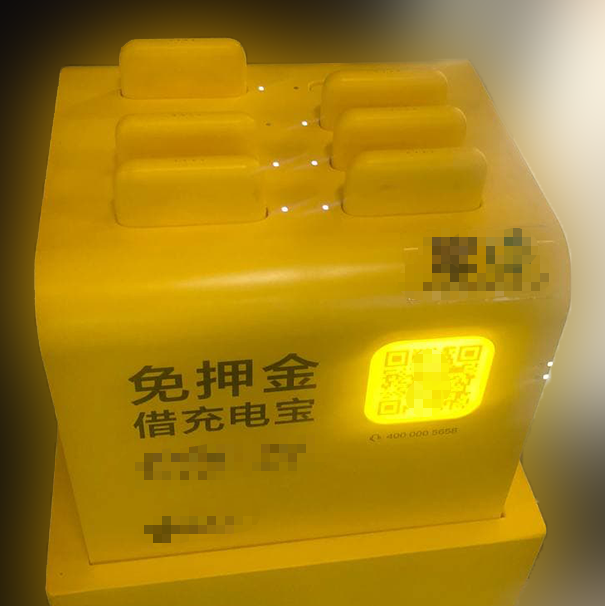
\includegraphics[width=.45 \linewidth, height=.45 \linewidth]{./Figs/PBS_mt.png}
	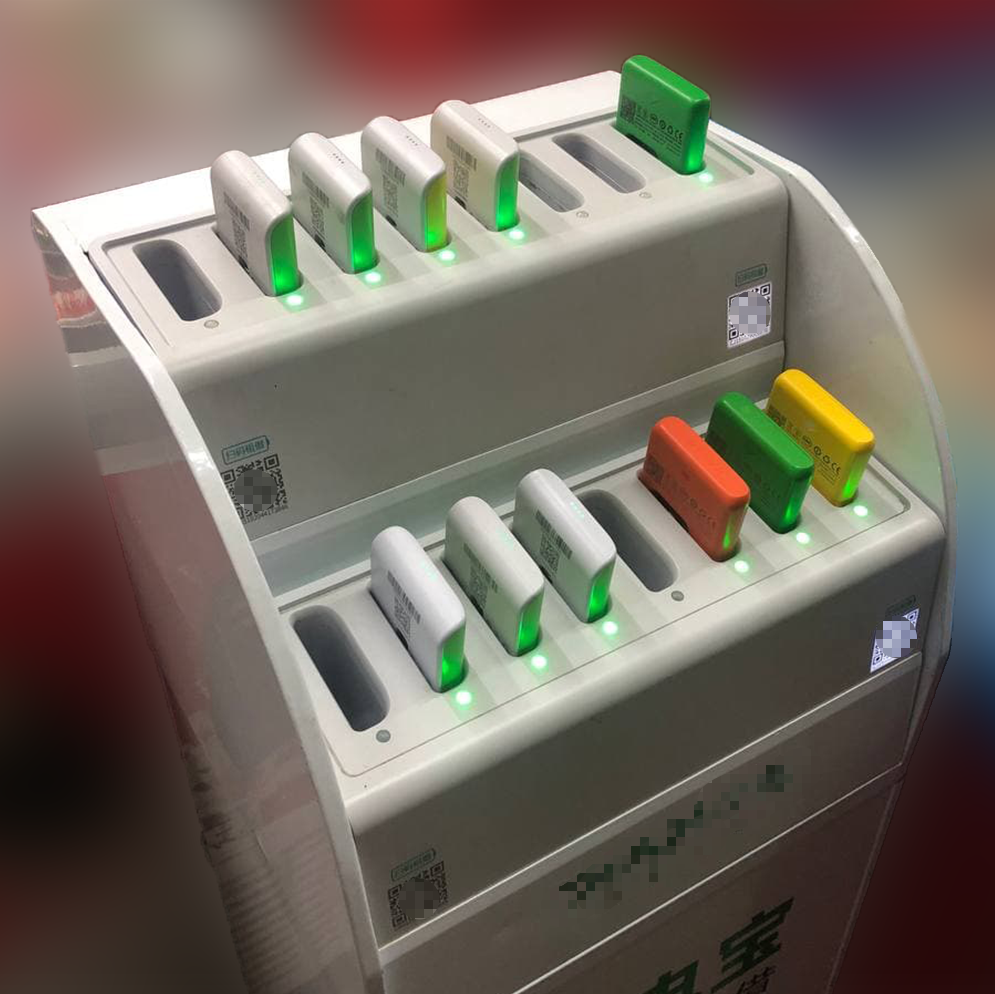
\includegraphics[width=.45 \linewidth, height=.45 \linewidth]{./Figs/PBS_xd.png}
	\caption{Two Power Bank Stations.}
	\label{fig:PBS_products}
\end{figure}

\DIFdelbegin \DIFdel{\shuqing{May use statistics (instead of concrete examples) to explain it.}
}\DIFdelend %DIF > \shuqing{May use statistics (instead of concrete examples) to explain it.}

Sharing power banks not only provides convenience to users, but also brings security issues.  We noticed that most of the power bank stations do not
check the integrity of power banks during the rental process, and users are
hardly cautious to check the power banks when connecting their devices.  An
attacker is able to tamper rented power banks and return them to a power bank
station causing a potential threat to subsequent users.


\textbf{QR Code Payment}.
QR code payment is a new type of payment method that is popular in Asia. Its most well-known cases are WeChat Pay~\cite{Wechat-pay} and Alipay~\cite{AliPay}. QR code payment provides merchant and client a convenient way of offline payment while ensuring equivalent security as the credit card.
As illustrated in Figure~\ref{fig:qr_payment_procedure},
 QR code payments are typically performed in the following steps:
\ding{182} The client presents the payment QR code on the mobile device to the merchant.
The QR code is encoded with a globally unique ID to identify the client's account.
\ding{183} The merchant scans the payment QR code and charges the corresponding amount of money.
By presenting this QR code, the client authorizes the proceeding transaction.
\ding{184} After confirmation, the payment service provider proceeds with this transaction and returns the payment result to both the merchant and the client.
\shuqing{I think this paragraph can be shorter. No need to explain so many details.}
\hongyi{Dont know how to be more concise.}

\begin{figure}[t]
	\centering
	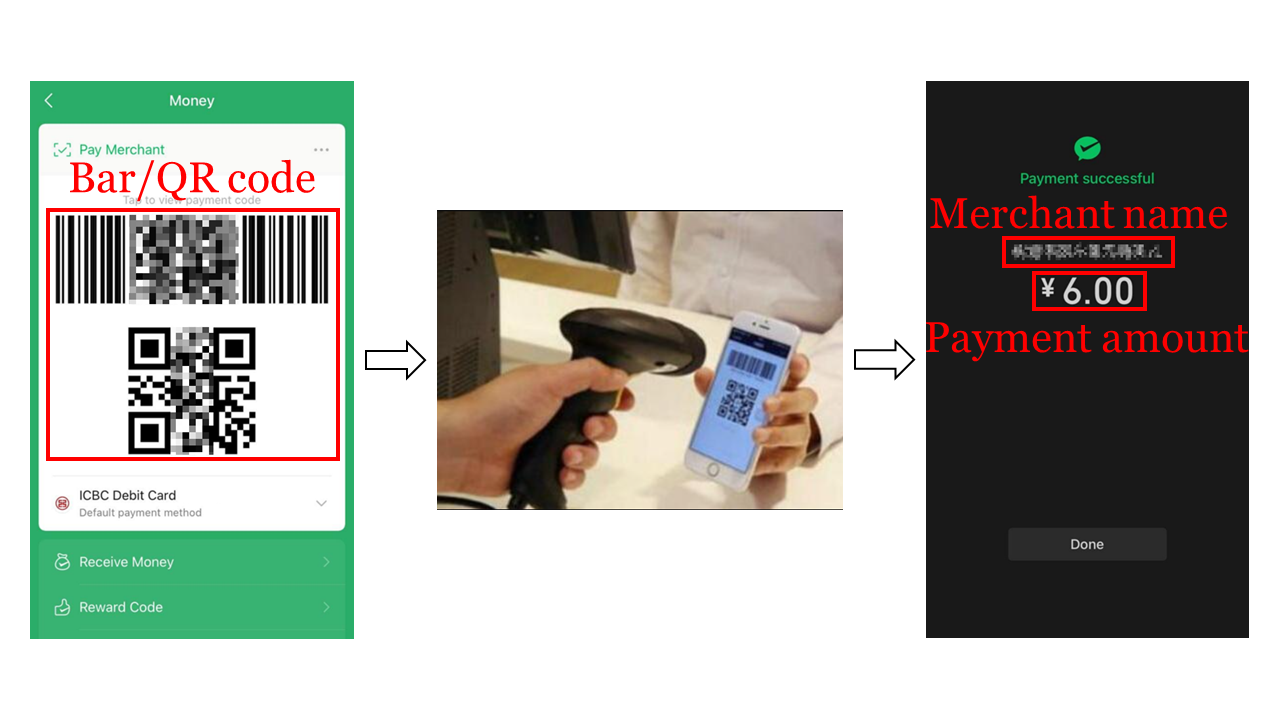
\includegraphics[width=\linewidth]{./Figs/qr_code_payment.png}
	\caption{Bar/QR Code Payment Procedure.}
	\label{fig:qr_payment_procedure}
\end{figure}


Next, we explain one type of payments called micropayment. A micropayment is pre-determined by the payment
service provider with thresholds in the user agreement. In real-world scenarios, payment service providers use different rules
for micropayment purchases. For example, WeChat
Pay~\cite{Wechat-pay} regards transactions under \DIFdelbegin \DIFdel{USD }\DIFdelend \DIFaddbegin \DIFadd{US}\DIFaddend \textdollar 154 as
micropayments.  Different from a typical payment procedure, when micropayments
are made, confirmations can be applied automatically without clients'
permission which aims to provide convenience to both merchant and client.  If a
victim's payment code is leaked to the attackers, they can use that code to
authorize multiple micropayments without needing permission.  In order to prevent such
cases, both WeChat Pay~\cite{Wechat-pay} and Alipay~\cite{AliPay} have designed a refreshing mechanism for the
payment code, which is to refresh the QR code every minute. This is sufficient
to stop an attack like opportunistic theft of a payment code but unable to stop a real-time attack like our
\tool.  In summary, the payment QR code is highly sensitive on users' devices
and our following case study is about how to obtain this code using an
attacker-crafted power bank via \tool.

\subsubsection{Attack Scenario}
\DIFaddbegin \label{subsec:attack-scenario}
\DIFaddend 

In this part, we will introduce a real-life attack scenario to show that our
\tool is a practical offensive tool.  This scenario can be broken down into the
following steps.

\begin{enumerate}[I. ]
	\item The attacker rents a power bank from one of the power bank stations and replaces the internal components with \tool.
	\item After the modification, an attacker-crafted power bank is returned to a rental station in a crowded area like an airport or railway station, which increases the probability of success.
	\item A user borrows the modified power bank and connects it to his/her own device, becoming the victim of \tool.
	\item The attacker now has complete control over the victim's device and can perform various attacks using different modes.
\end{enumerate}

Next, we summarize the possible threats toward users under different modes.
%\hongyi{Better way to express this?}
First, under \ac{HID} emulator mode, the attacker is able to implant malware and backdoor scripts into victims' devices. Moreover, using video capture mode, once the victims access their sensitive data such as QR payment  code or photos, their sensitive data \DIFdelbegin \DIFdel{will }\DIFdelend \DIFaddbegin \DIFadd{could }\DIFaddend be immediately transmitted via \tool to the attacker. Lastly, with full control mode, the attacker has complete control over the victims' \DIFdelbegin \DIFdel{device and can conduct any action on the victim device}\DIFdelend \DIFaddbegin \DIFadd{devices and could conduct any actions on the victims' devices}\DIFaddend .

\shuqing{Background is longer than real user study.}
%As the functionality and effectiveness, HID emulator mode is similar to the original BadUSB and the full control mode hijacks the victim's device completely.
\hongyi{I dont know if it's a good enough reason}
%Here we only validate the usability of privacy extraction mode and conducted a user study.

\DIFdelbegin \DIFdel{To further validate our attacking scenario , we invited 10 volunteers, who are students in our university, to participate and conduct a user study.
Before the user study experiment, we disclosed to the volunteers how their data might be used and request permission from the volunteers and the university ethics review boards.
During the case study, volunteers took turns to use their phones for half an hour with }\DIFdelend \DIFaddbegin \subsubsection{\DIFadd{Experiment}}

\DIFadd{We conducted experiments to further validate the capabilities of }\DIFaddend \tool 
\DIFdelbegin \DIFdel{connected. 
To obtain data close to real-life, they were requested to use phones just as they were normally using sharing power banks.
At the same time, we used scripts to perform }%DIFDELCMD < \ac{OCR} %%%
\DIFdel{recognition for each frame in the videos stream and stored all of the }%DIFDELCMD < \ac{OCR} %%%
\DIFdel{results in a database}\DIFdelend \DIFaddbegin \DIFadd{in the attack scenario introduced in Section~\ref{subsec:attack-scenario}.
11 applications were selected and tested on \mbox{\textit{HUAWEI P30 (ELE-AL00)}} step by step:
(1) Login in with a test account.
(2) Keep the default settings.
(3) Attach attacker's }\tool \DIFadd{to the test device.
(4) Simulate victim's daily usage of the application}\DIFaddend .

\DIFdelbegin \DIFdel{After each experiment, the raw video and the corresponding }%DIFDELCMD < \ac{OCR} %%%
\DIFdel{result file was generated automatically, then we presented these files to him/her, introduced our attack, told him/her to analyze the video file and replace certain characters of the private data that appear in the }%DIFDELCMD < \ac{OCR} %%%
\DIFdel{result file with asterisks. This protects their privacy and is also a mark for us to confirm thatthe data we find contains their private data. At last, he/she would destroy all original files, leave only the desensitized }%DIFDELCMD < \ac{OCR} %%%
\DIFdel{results for us. 
%DIF < \shuqing{Do we need to mention that agreement the conference required here?}
%DIF < \hongyi{I'm also quite concern about this.}
}%DIFDELCMD < 

%DIFDELCMD < %%%
\subsubsection{\DIFdel{Result}}
%DIFAUXCMD
\addtocounter{subsubsection}{-1}%DIFAUXCMD
%DIFDELCMD < 

%DIFDELCMD < %%%
\DIFdel{In total, there are 94}\DIFdelend \DIFaddbegin \DIFadd{During this experiment, we tested full control mode which actively obtained sensitive information and video capture mode which passively obtained the sensitive information visited by the victim. We noticed that}\DIFaddend , \DIFdelbegin \DIFdel{058 entries of data from 10 volunteers. An entry is a combination of the case number, the frame number and the desensitized }%DIFDELCMD < \ac{OCR} %%%
\DIFdel{result.
%DIF < \shuqing{The data may need to be updated.}
With these results, we could learn what content the victimvisited, especially the privacy data.
%DIF < \fengwei{The following text needs to be revised. It is quite difficult for me to understand. Note that this is important text because reviewers are curious about the result. }
We searched the result database with the keywords }\textit{\DIFdel{account, username, password, phone number and email}}%DIFAUXCMD
\DIFdel{, as well as the regular expression of email.
The records searched by such keywords and regular expressions are usually related to privacy information of users}\DIFdelend \DIFaddbegin \DIFadd{most sensitive information could be obtained directly through full control mode without victim's interaction, but there was also certain information that had to be obtained passively through video capture mode}\DIFaddend . For example, \DIFdelbegin \DIFdel{when we searched with }\textit{\DIFdel{account}} %DIFAUXCMD
\DIFdel{as a keyword, victim's accounts could be found in the database, as shown in the Table~\ref{tab:ocr_keyword_example} and Table~\ref{table:information_extracted}.
%DIF < \shuqing{Statistics.}
At last, we found 4, 172 of 94}\DIFdelend \DIFaddbegin \DIFadd{as illustrated in Table~\ref{table:information_extracted}}\DIFaddend , \DIFdelbegin \DIFdel{058 records obtained by }%DIFDELCMD < \tool %%%
\DIFdel{which are related to privacy information , as shown in the Table~\ref{table:information_extracted}}\DIFdelend \DIFaddbegin \DIFadd{in most applications, information like ``Account'' can be obtained directly while information like ``Payment Password'' cannot be obtained until the victim inputs his/her password}\DIFaddend .

\DIFaddbegin \subsubsection{\DIFadd{Result}}
\DIFaddend In summary, \DIFdelbegin \DIFdel{though we cannot directly obtain the user's password on the lock screen, we can still check all of the information presented on the screen, extract sensitive information including but not limited to social accounts, bank accounts, personal financial situation, etc., if the user unconsciously unlocks the screen.
It is worth mentioning that }%DIFDELCMD < {%%%
\DIFdel{secure keyboards}%DIFDELCMD < } %%%
\DIFdel{built in financial apps show their keyboard typing sequences, which can be easily captured by }\DIFdelend \tool \DIFdelbegin \DIFdel{.
}\DIFdelend \DIFaddbegin \DIFadd{is able to actively obtain most sensitive information from the screen, such as browsing history, personal account, phone number without victim's interaction. There also exists information such as payment password that is not available immediately, but such a piece of information can be obtained once the victim inputs it. The obtained information can be used to guess the victim's lock screen password and poses further threat to victim's privacy.
}\DIFaddend 

\DIFaddbegin \begin{table*}[t]
	\centering
	\begin{tabular}{|c|c|l|l|c|c|}
		\hline
		\multirow{2}{*}{\textbf{Category} } & \multirow{2}{*}{ \textbf{Application} } & \multicolumn{2}{c|}{\textbf{Leaked Sensitive Information}} \\
															\cline{3-4}
											&				& \textbf{\DIFaddFL{Without Victim's Interaction}}						& \textbf{\DIFaddFL{With Victim's Interaction}} \\
		\hline
		\DIFaddFL{Social \& Finance App 				}& \DIFaddFL{WeChat (8.0.1)      }& \DIFaddFL{Account, Financial Status, Chat History, Payment Code   		}& \DIFaddFL{Payment Password }\\
		\hline
		\multirow{2}{*}{Social App}
											%DIF > & QQ          & Account, Contacts, Chat History   	& \\
											%DIF > \cline{2-4}
							       			& \DIFaddFL{WhatsApp (2.21.5.18)    }& \DIFaddFL{Account, Contacts, Chat History, Phone Number    }& \\
											\cline{2-4}
							       			& \DIFaddFL{Facebook (309.0.0.47.119)   }& \DIFaddFL{Account, Posts, Contacts           }& \\
		\hline
		\multirow{3}{*}{Finance App}       	& \DIFaddFL{Alipay (10.2.15.9500)      }& \DIFaddFL{Account, Financial Status, Payment Code         				}& \DIFaddFL{Payment Password }\\
											\cline{2-4}
											& \DIFaddFL{Cash App (3.35.1)   }& \DIFaddFL{Email, Phone Number, Cash Balance							}& \DIFaddFL{Payment Password }\\
											\cline{2-4}
											& \DIFaddFL{Paypal (7.38.1)      }& \DIFaddFL{Account, PayPal Balance     								}& \DIFaddFL{Payment Password }\\
		\hline
		\multirow{1}{*}{Shopping App}		& \DIFaddFL{Amazon Shopping (22.6.0.100)  }& \DIFaddFL{Account, Orders, Shopping Cart         				}& \\
											%DIF > \cline{2-4}
		                					%DIF > & Taobao      & Personal physical metrics      						& \\
		\hline
		\multirow{2}{*}{Tool}               & \DIFaddFL{Chrome (89.0.4389.72)      }& \DIFaddFL{Browsing History                                	}& \\
											\cline{2-4}
		                					& \DIFaddFL{Health (11.0.5.508)      }& \DIFaddFL{Personal Health Metrics      						}& \\
		\hline
		\multirow{3}{*}{System}             &  \DIFaddFL{Messages (11.0.1.430)   }& \DIFaddFL{Contacts, Chat History				 }&   \\
											\cline{2-4}
											& \DIFaddFL{Settings (11.0.0.300) - WiFi   }& \DIFaddFL{WiFi SSID                                	}&  \DIFaddFL{WiFi Password }\\
											\cline{2-4}
		                					& \DIFaddFL{Settings (11.0.0.300) - VPN    }& \DIFaddFL{VPN Address, VPN Account, VPN Password      						}& \\
		\hline
	\end{tabular}
	\linebreak
	\caption{\DIFaddFL{Sensitive Information Leaked From Applications.}}
	\label{table:information_extracted}
\end{table*}


%DIF > %%%%%%%%%%%%%%%%%%%%%%%%%%%%%%%%%%%%%%%%%%%%%%%%%%%%%%%%%%%%%%%%%%%%%%%%%%%%%%%%%%%%%%%
%DIF >  It is unfortunate that the user study is not part of the paper anymore.

\DIFaddend \section{Countermeasures}
\label{sec:countermeasures}

%Authorization mechanisms like GoodUSB~\cite{tian2015defending} have been
%proposed as countermeasures against BadUSB attacks. As mentioned in
%Section~\ref{sec:badusb} and Section~\ref{sec:experiment}, GoodUSB relies on
%internal display for authorization, which can be bypassed via our \tool. 
%Hence, GoodUSB is indeed a great defense against traditional BadUSB attack but
%no defense at all for our \tool. 
Next, we discuss our recommended countermeasures against \tool.

\textbf{External Hardware Authorization.} One possible countermeasure is to
introduce external hardware completing the authorization process. For example,
 \mbox{USBCheckIn}~\cite{usbcheckin} adopts a dedicated hardware between
the host and device. When a device is plugged-in, the authorization will be
conducted on the dedicated hardware instead of the internal display, preventing
the host from being hijacked. Although \mbox{USBCheckIn} is an adequate defense against
\tool, the external hardware brings additional cost and inconvenience,
especially for mobile devices.

\textbf{Distrust-by-Default.} Most security issues of \ac{USB} protocol are due to
its \textit{trust-by-default} assumption; \tool also relies on this feature to work.
To defend against \tool and other USB-based attacks, we can simply reject all
{unauthorized} \DIFdelbegin \DIFdel{device }\DIFdelend \DIFaddbegin \DIFadd{devices }\DIFaddend -- applying the \textit{distrust-by-default} policy. For example, 
in GoodUSB~\cite{tian2015defending}, all \ac{USB} devices are enabled with corresponding 
functionality only after being authorized by the user. 
Defense like USB Condom distrusts all types of \ac{USB} devices by blocking data channels and stopping all \ac{USB} functions other than charging.
Such defense methods effectively stop attacks 
like \tool.

\textbf{Isolated \ac{UI} Rendering.} During our experiments, we noticed that \tool
is actually unable to mirror the lock screen keyboard from the iPad
OS. Instead, the keyboard is only available on the internal display. However,
this defense is only enabled on the lock screen keyboard, other keyboards
(e.g., the virtual ones used by the apps) are still vulnerable to our \tool.
This mechanism has inspired us to propose a new defense against our \tool
called \emph{Isolated \ac{UI} Rendering}. As illustrated in
Figure~\ref{fig:isolated_ui}, we designed two separated \ac{UI} render layers and corresponding drivers, one
is secure the \DIFdelbegin \DIFdel{other }\DIFdelend \DIFaddbegin \DIFadd{another }\DIFaddend is insecure. When an application requires to render, it can
pass the content along with a tag identifying whether the content is
``sensitive'' or not. If the content is tagged with ``sensitive'', then the OS
\DIFdelbegin \DIFdel{will }\DIFdelend \DIFaddbegin \DIFadd{could }\DIFaddend only render it on the secure layer, which only shows the sensitive content
(e.g., a keyboard) on the trusted screen. For the rest of the rendering, it
would render on both the trusted and untrusted display (e.g., insensitive
contents).
For example, in Figure~\ref{fig:isolated_ui}, the ``password'' and ``keyboard'' are recognized as sensitive while other parts of content are insensitive. Thus, the ``password'' and ``keyboard'' are not rendered on untrusted screen.

\begin{figure}[t]
	\centering
	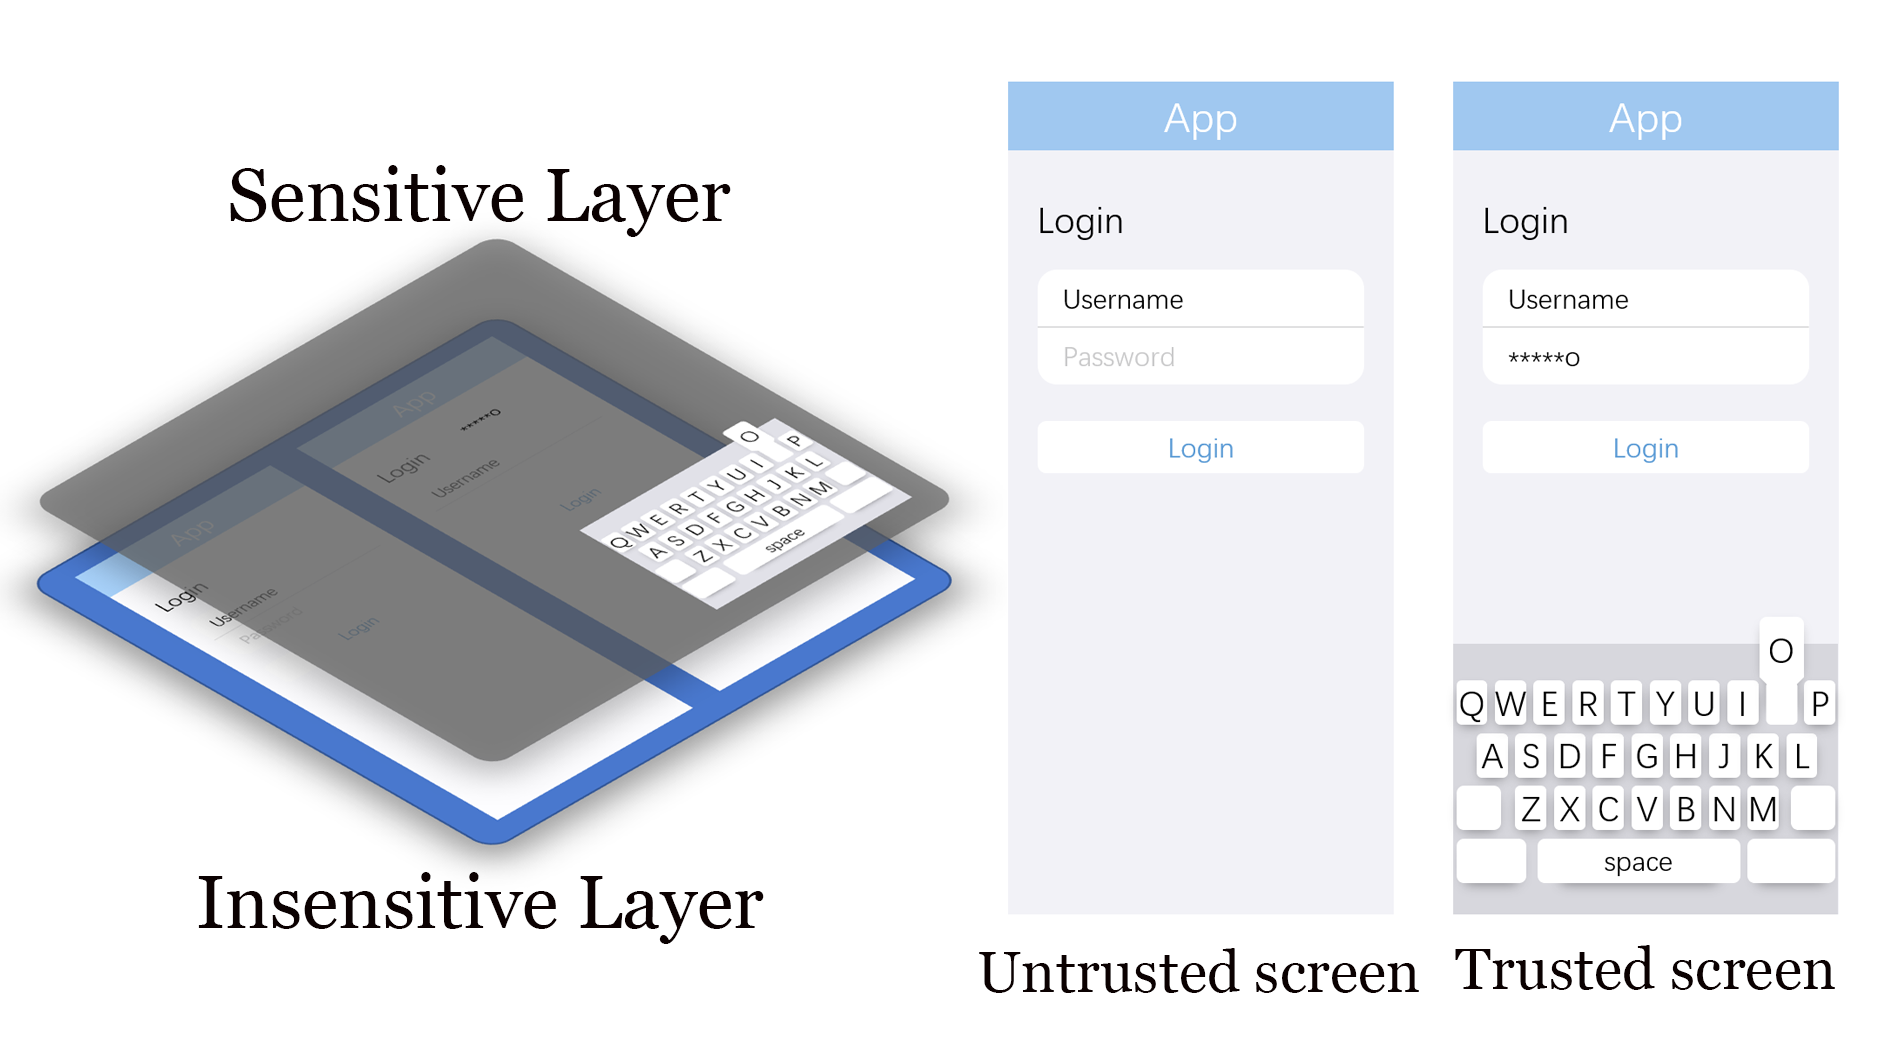
\includegraphics[width=\linewidth]{./Figs/isolated_ui.png}
	\caption{Isolated \ac{UI} Rendering}%\shuqing{Maybe we can increase the font?}
	\label{fig:isolated_ui}
\end{figure}
%\fengwei{what are untrusted and trusted screens? are they internal and external displays?}
%\hongyi{Fixed by using the same term and additional description}

\section{Discussion}
\label{sec:discussion}

\subsection{Limitation}
There exist multiple limitations of \tool. To begin with, when \tool is attached, the victim's device may not be set to mirror the screen. 
Depending on the victim's settings, the \tool may be used as an extended monitor or \DIFaddbegin \DIFadd{be set to `Desktop Mode' or }\DIFaddend not be enabled at all. \DIFdelbegin \DIFdel{Additionally, some smartphone vendors (e.g. Huawei and Smartisan) provide a Desktop Mode to users, which displays a desktop on external screeninstead of mirroring}\DIFdelend \DIFaddbegin \DIFadd{Though we proposed the attack initialization in Section~\ref{subsec:attack_init} to inject keystrokes to ensure }\tool \DIFadd{is mirroring primary screen. But without knowing the exact operating system of the victim's device, }\tool \DIFadd{may have to try multiple injections before successfully mirroring the screen}\DIFaddend .
Moreover, as mentioned in Section~\ref{sec:experiment}, \tool cannot directly obtain the information on the lock screen.
 \DIFdelbegin \DIFdel{In these cases, }%DIFDELCMD < \tool %%%
\DIFdel{is either easily noticeable to the victim or disabled.  }\DIFdelend Apart from that, we also noticed that in most devices, when an external monitor is connected to the device, there will be notifications about the monitor. In iPad, there is a small blue icon on the notification bar. In Windows 10, there is a pop-up for user to select the functionality of the external monitor. In latter case of a pop-up, \tool can dismiss it by injecting keystrokes \DIFdelbegin \DIFdel{and mouse movements}\DIFdelend \DIFaddbegin \DIFadd{as described in Section~\ref{subsec:attack_init}}\DIFaddend . But they are still noticeable by the victim. Also, it cannot be ignored that DisplayPort over \ac{USB} is not available on all devices. When selecting devices to test \tool, we find that many smartphones equipped with USB-C connectors \DIFaddbegin \DIFadd{actually }\DIFaddend do not support \ac{USB} \DIFdelbegin \DIFdel{3.2 protocol. Such lack of support further limits }%DIFDELCMD < \tool%%%
\DIFdel{. }\DIFdelend \DIFaddbegin \DIFadd{3.x protocol. There is a incomplete list of devices that support DisplayPort over }\ac{USB}\DIFadd{~\mbox{%DIFAUXCMD
\cite{usbclist}}\hspace{0pt}%DIFAUXCMD
. Most vendors like HUAWEI and Samsung tend to support }\ac{USB} \DIFadd{3.x protocol in their \mbox{high-end} smartphones. But there also exists vendor like Xiaomi who does not support }\ac{USB} \DIFadd{3.x protocol at all. 
}\DIFaddend 

\begin{comment}
There exist multiple limitations of \tool.  To begin with, \tool can only gain
the information and control access of the host itself instead of external
hardware.  Consequently, as we introduced in the
Section~\ref{sec:countermeasures}, \tool can hardly bypass the defense
approaches that use external hardware for authorization.  Moreover, most of
the devices will prompt users to give authentication to the \ac{USB} devices or
select one of the functional modes after they are plugged in.  Though some of
such prompts are not conspicuous for non-experts, especially when \tool is
concealed within other functional hardware such as power banks \shuqing{If
there is experiment, add it here.}, the probability of whether users could get
aware that something unusual happens will increase with the existence of these
prompting messages.
\end{comment}
\subsection{Impact}

%\shuqing{Left after experiment to finish. Will discuss from different modes
%and application scenarios.}
The \ac{USB} protocol is used widely as introduced in the preceding sections.  As the
technologies develop rapidly, more and more devices will be equipped with USB-C
capabilities\DIFaddbegin \DIFadd{~\mbox{%DIFAUXCMD
\cite{li2018usb}}\hspace{0pt}%DIFAUXCMD
}\DIFaddend , which makes \tool more influential.  
Since non-professional users \DIFdelbegin \DIFdel{often }\DIFdelend \DIFaddbegin \DIFadd{may }\DIFaddend neglect checking the security of plug-in \ac{USB} devices, 
they \DIFdelbegin \DIFdel{are often }\DIFdelend \DIFaddbegin \DIFadd{may }\DIFaddend unaware of the attacks from \tool.
can be hardly detected by them while attacks are performing.  
The popularity and universality of public \ac{USB} devices, including sharing power banks, even
increase such risks.  Moreover, \tool provides a better way for traditional
BadUSB attacks, since attackers can obtain the screen streaming with ease.
Attackers can use such technologies to perform more precise attacks, such as
interacting with the user interface and controlling the consequences of their
attacks.  In summary, \tool can be applied in various application scenarios and
brings rather huge impacts.

\section{Conclusion}
\label{sec:conclusion}
\outline{Conclusion}

Leveraging the new features of \ac{USB} 3.x~\cite{usb30,usb31,usb32}, we explore a
new attack scheme named \tool and three attack modes. Each of these three modes
has its own strength and use scenarios. The \ac{HID} Emulation mode largely extends the
original BadUSB. The video capture mode proved practical and powerful\DIFdelbegin \DIFdel{in the user study}\DIFdelend , as it extracts
victim's sensitive information in a stealthy way. The fully control mode
achieves the complete hijack of the target device, allowing us to perform various
types of subsequent attacks. By experimenting \tool with mobile phones, tablets,
and PCs, we further test its ability under different modes. In our \DIFdelbegin \DIFdel{user study}\DIFdelend \DIFaddbegin \DIFadd{experiment}\DIFaddend , we
obtain and analyze video stream extracted from \DIFdelbegin \DIFdel{10 participants }\DIFdelend \DIFaddbegin \DIFadd{11 applications }\DIFaddend with \tool,
which demonstrates its capability in a \DIFaddbegin \DIFadd{simulated }\DIFaddend real-life scenario. In the end, we
propose a new defense scheme named \textit{isolated UI rendering}, which can
effectively stop \DIFdelbegin \DIFdel{our }\DIFdelend \DIFaddbegin \DIFadd{attacks with }\DIFaddend \tool.
\DIFdelbegin %DIFDELCMD < 

%DIFDELCMD < %%%
\DIFdelend As for future work, we will further explore the potential of \textit{isolated UI
rendering} and implement it on a customized operating system. Moreover, we also
hope to lower the power consumption for network transmission in \tool to make
it more practical.

\section{Responsible Disclosure}
\DIFdelbegin %DIFDELCMD < 

%DIFDELCMD < %%%
\DIFdelend Responsible disclosure have already been carried out, we have \DIFdelbegin \DIFdel{already contacted Huawei }\DIFdelend \DIFaddbegin \DIFadd{contacted HUAWEI }\DIFaddend and Apple through proper \DIFdelbegin \DIFdel{channel and are waiting for mitigation being deployed. We revived response from Huawei on }%DIFDELCMD < \nth{7} %%%
\DIFdel{March and discussed about }\DIFdelend \DIFaddbegin \DIFadd{channels. We received response from HUAWEI on March }\nth{7} \DIFadd{and discussed }\DIFaddend the mitigation plan on \DIFdelbegin %DIFDELCMD < \nth{10} %%%
\DIFdel{March }\DIFdelend \DIFaddbegin \DIFadd{March }\nth{10} \DIFaddend while Apple has not responded yet. \DIFaddbegin \DIFadd{HUAWEI security team has confirmed this issue and been working on mitigation. We are actively facilitating their mitigation process and waiting for a fix to be deployed. After the mitigation is deployed, HUAWEI will assign a CVE ID for this vulnerability.
}

\section{\DIFadd{Acknowledgement}}
\DIFadd{We are very grateful to our shepherd, Michael Schwarz, and the anonymous reviewers for their valuable feedback that improved the paper.
}\DIFaddend %\input{./Files/acknowledgement.tex}





\balance




\end{document}
